\documentclass[preprint, 11pt]{elsarticle}
\usepackage{geometry}
\geometry{top=1in, left=1.3in,right=1.3in,bottom=1in}

\usepackage{booktabs,calc,soul,xcolor}
\setstcolor{red}

\usepackage{marginnote} 
% Marginpar width
%Marginpar width
\newcommand{\pts}[1]{\marginpar{ \small\hspace{0pt} \textit{[#1]} } }
\setlength{\marginparwidth}{1.1in}


%\reversemarginpar
%\setlength{\marginparsep}{.02in}

%% Fonts
% \usepackage{fourier}
% \usepackage[T1]{pbsi}

\usepackage{lmodern}
\usepackage[T1]{fontenc}
%\usepackage{minted}

\usepackage{rotating}
\usepackage{amsmath, amssymb}
%% Cite Title
%\usepackage[style=numeric,backend=biber,sorting=none,maxcitenames=2,maxbibnames=99,doi=false,isbn=false,url=false,eprint=false]{biblatex}
%\addbibresource{references.bib}

%\usepackage{lineno}
%\renewcommand\linenumberfont{\normalfont\small}
%\linenumbers



\usepackage{graphicx}
\graphicspath{{./images/}}
 
\usepackage{rotating}
\usepackage{longtable}

%\usepackage{enumerate}
\usepackage{paralist}
\usepackage{epstopdf,subfigure,hyperref,enumerate,polynom,polynomial}
\usepackage{multirow,minitoc,fancybox,array,multicol}

% \definecolor{slblue}{rgb}{0,.3,.62}
% \hypersetup{
%     colorlinks,%
%     citecolor=blue,%
%     filecolor=blue,%
%     linkcolor=blue,
%     urlcolor=slblue
% }


%%%TIKZ
\usepackage{tikz}
\usepackage{pgfplots}
\usepackage{pgfplotstable}
\usepackage{pgfgantt}
\pgfplotsset{compat=newest}

\usetikzlibrary{arrows,shapes,positioning,shapes.geometric}
\usetikzlibrary{decorations.markings}
\usetikzlibrary{shadows,automata}
\usetikzlibrary{patterns}
\usetikzlibrary{trees,mindmap,backgrounds}
%\usetikzlibrary{circuits.ee.IEC}
\usetikzlibrary{decorations.text}
\usetikzlibrary{ decorations.pathreplacing,decorations.pathmorphing}
\tikzset{no shadows/.style={general shadow/.style=}}

% Default fixed font does not support bold face
\DeclareFixedFont{\ttb}{T1}{txtt}{bx}{n}{8} % for bold
\DeclareFixedFont{\ttm}{T1}{txtt}{m}{n}{8}  % for normal


\newcommand{\osn}{\oldstylenums}
\newcommand{\dg}{^{\circ}}
\newcommand{\lt}{\left}
\newcommand{\rt}{\right}
\newcommand{\pt}{\phantom}
\newcommand{\tf}{\therefore}
\newcommand{\?}{\stackrel{?}{=}}
\newcommand{\fr}{\frac}
\newcommand{\dfr}{\dfrac}
\newcommand{\tn}{\tabularnewline}
\newcommand{\nl}{\newline}
\newcommand\relph[1]{\mathrel{\phantom{#1}}}
\newcommand{\cm}{\checkmark}
\newcommand{\ol}{\overline}

%%% COLORS %%%%
\newcommand{\rd}{\color{red}}
\newcommand{\bl}{\color{blue}}
\newcommand{\pl}{\color{purple}}
\newcommand{\og}{\color{orange!90!black}}
\newcommand{\gr}{\color{green!40!black}}
% Custom colors
%\usepackage{color}
\definecolor{deepblue}{rgb}{0,0,0.5}
\definecolor{deepred}{rgb}{0.6,0,0}
\definecolor{deepgreen}{rgb}{0,0.5,0}


%%% FORMATTING MACROS %%%%%
\newcommand{\nin}{\noindent}
\newcommand{\la}{\lambda}
\renewcommand{\th}{\theta}
\newcommand{\al}{\alpha}
\newcommand{\G}{\Gamma}
\newcommand*\circled[1]{\tikz[baseline=(char.base)]{
    \node[shape=circle,draw,thick,inner sep=1pt] (char) {\small #1};}}

\newcommand{\bc}{\begin{compactenum}[\quad--]}
\newcommand{\ec}{\end{compactenum}}

\newcommand{\p}{\partial}
\newcommand{\pd}[2]{\frac{\partial{#1}}{\partial{#2}}}
\newcommand{\dpd}[2]{\dfrac{\partial{#1}}{\partial{#2}}}
\newcommand{\pdd}[2]{\frac{\partial^2{#1}}{\partial{#2}^2}}

\journal{Journal Name}

\begin{document}
 
 
\begin{frontmatter}
  
\title{Investigating country-level activity and mobility patterns  and their interdependencies on COVID-19 outcomes}


\author[umass]{Atanas Apostolov}
\author[umass]{Jimi B.\ Oke} 
 
\address[umass]{Department of Civil and Environmental Engineering, University of Massachusetts Amherst, MA 01003, United States}


\begin{abstract}
In this paper we examine the effects of COVID-19 on mobility, segmented by transportation type, as well as social activity such as retail and recreation, workplaces and residential, and their interdependencies.
Using time series data from 63 countries across five continents,
we investigate patterns in activity and mobility trends from mid-February through August.
Our findings yield insights into how various activities have been impacted by COVID-19 and vice-versa.
\marginnote{\scriptsize\rd We will revisit the abstract once the manuscript itself is done.}
\end{abstract}

\begin{keyword}
  COVID-19 \sep mobility \sep vector autoregression
\end{keyword}

\end{frontmatter}

\section{Introduction}
\textit{\bl This section sets up the motivation and significance of the work presented in this paper. Key questions:
  \begin{enumerate}
  \item What is the ongoing and potential future impact of COVID-19 across various countries, particularly on mobility and activity patterns? What are the implications (known and unknown)?
  \item Briefly what has been done in terms of modeling mobility impacts?
  \item Where are the current gaps in our knowledge?
  \item (Final paragraph) What is the summary of this paper's contributions? What is the expected significance of our results?
  \end{enumerate}
}


\marginnote{\scriptsize\rd I want to you to focus your near-term writing efforts on the Introduction, Relevant Work
  (Literature Review) and Data and Methods (Sections 3.1 and 3.2) }
COVID-19 has had a severe impact on mobility and social activities since initial reports of the disease emerged in late 2019.
By May 2020 most countries had implemented social distancing measures and imposed strict travel restrictions to curtail the spread of the virus
both within their borders and internationally.
According to \cite{bonaccorsi2020economic}, the international spread of the disease can be partially explained by risk perception,
mobility behavior and social media influences using a global vector autoregression (GVAR) modeling framework\cite{dees2007exploring}.
%Milani concludes that most countries learn from each other's social distancing response which can be partially explained by social networks.  
\cite{zhang2020pathways} confirm that human mobility is key to understanding the transmission pathways.
Using a mobility dataset of over 500,000 flights and over 100 million passengers,
the authors develop a dynamic network model using time-dependent border restrictions as exogenous variables.
\cite{mckenzie2020country} studied the patterns in 6 activity responses across 108 countries but this was an exploratory effort in comparison with government policies and it included no modeling attempt to explain COVID-19 outcomes.

Beyond these global studies, several city and country-specific simulations and models have been estimated to explain how activities, mobility (particularly transit) impact COVID-19 outcomes.
\cite{kumar2020activitybaseda} used an activity-based epidemiological framework to study how COVID-19 is propagated across various daily activities in car-dependent cities typically found in the US and Canada.
They quantified the effect of the transit network on COVID-19 spread and demonstrated the importance of work and home activities in the early and latter stages of the epidemic.
\cite{badr2020association} developed a generalized linear model to explain COVID-19 growth based on overall mobility changes at the county level in the US. Inter-county movements were factored in but impacts by mode or activity were not analyzed.
Given China's and then  Italy's prominence in the earlier stages of the pandemic, several studies have examined their mobility patterns \cite{
  kraemer2020effect,bonaccorsi2020economic,pepe2020covid19,carteni2020how}.
While these have been important for country-wide epidemiological studies, they have not provided knowledge on activity-based impacts.

Therefore, there remains an urgent need to understand the interdependencies between COVID-19 outcomes and human mobility and activity patterns.
Statistically significant models can yield insights to enable policymakers contain and recover from the ongoing pandemic.
Furthermore, these models can guide future decisions in containing the spread of future epidemics.
In this paper, we conduct a global scale country-level analysis of COVID-19 infections,  mobility and activity patterns.
First, we cluster the countries to discover patterns in mobility and activity changes.
Second, we estimate cluster-representative models using the vector autoregression (VAR) framework, allowing for time lags across all endogenous variables, and thus including dynamic interdependencies among them.
These models explain which activities impact COVID-19 outcomes and vice versa, providing potential pathways for understanding behavioral responses to the spread of the pandemic and a greater understanding of the disparities and similarities across nationwide outcomes.



\section{Relevant work}
\subsection{Modeling the activity and mobility impacts of COVID-19}

\hl{Summarize efforts to analyze activity-mobility patterns historically and now in the context of
  COVID-19, and then}
  
\subsection{Global vector autoregression}
\hl{Brief history and application of G/VAR modeling to date (in all areas - chiefly macroeconomic). I can help a bit
  here, but this is a critical section. It will also help you consolidate your grasp of GVAR developments to date.}

\section{Data and Methods}
\hl{Provide a preamble summarizing what this section entails.}

\subsection{Data sources and variables}
We use four disparate data sources in performing our COVID-19 mobility analysis. The endogenous category represents the variables in our model which we aim to predict. It covers daily COVID-19 counts, a global data set of new confirmed cases and deaths provided by Johns Hopkins University\footnote{\url{https://github.com/CSSEGISandData/COVID-19}}, as well as an activity benchmark – movement trends tracked by Google which are segmented by geographic region and type such as residential, workplace and transit. Google’s Community Mobility reports capture aggregated location data for a variety of categorized places from February 15 to August 31. 

The Google data set\footnote{\url{https://www.google.com/covid19/mobility/}} reveals the change in the number of visitors from that period compared to a pre-COVID baseline (January 3 – February 6, 2020). Google tracks actual foot traffic for their Reports which is reflective of the trips taken in each country. In contrast, Apple offers a snapshot of user requests made on its Apple Maps web service which constitutes hypothetical traffic and is not the focus of this research. However, the set of countries with available Apple Maps data influenced the geographic distribution in our analysis due to higher technological development in these areas.

The exogenous category represents measures implemented by governments worldwide in response to the pandemic and is put together by ACAPS – a non-profit project based in Geneva, Switzerland – along with the United Nations and other sources. The exogenous variables are external to the model.

The deterministic category spans a range of world development indicators tracked by the World Bank. The variables included in this model are primarily demographic and economic, measuring population growth and GDP. Unlike the endogenous and exogenous data sets which are presented in a time-series format, deterministic variables are collected for a single year (2015).

Finally, we utilize a flight data set measuring the number of incoming and outgoing flights from a specified set of countries. This data set is used to calculate a country-specific weight matrix passed as an argument to the GVAR model. The flight data is obtained from the travel data intelligence agency Airsavvi. 

The sources are summarized in \autoref{tab:sources} and the variables are described in \autoref{tab:variables}. The integrated dataset (along with the code and plots generated for this paper) is publicly available on Github.\footnote{\url{https://github.com/narslab/covid-analysis/tree/master/mobility}}


\begin{table}[h!]
  \centering
  \caption{Summary of data sources}
  \label{tab:sources}
  \footnotesize
\begin{tabular}{ll}\toprule
\bf Source                         		         & \bf Overview                                                                              \\\midrule
Johns Hopkins University          	         & New COVID cases and COVID-related deaths \\
  & (global time series summary)                                                              \\
Google Community Mobility Reports      & Change in traffic compared to a baseline day \\
  & (median value over period from Jan 3 to Feb 6, 2020) 			\\
World Data Indicators 		         & Economic indicators (growth, GDP) \\
Government Measures		         & ACAPS Government Measures Dataset \\\bottomrule
\end{tabular}
\end{table}
\marginnote{\scriptsize\rd Table 1 is OK, but with the expanded version of Table 2 I'm suggesting, it may no longer
  be necessary. In any case, put the citations into the table as well.}

\begin{table}[h!]
  \caption{Summary of variables used in GVAR model}
  \label{tab:variables}
  \footnotesize
  \centering
  \begin{tabular}{l l l l l}\toprule
    \textbf{Category} &  \textbf{Variable} & \textbf{Description}  & \textbf{Type} &  \textbf{Source}\\\midrule
    \multirow{8}{.8in}{Endogenous}
  & case     & infections            & \multirow{2}{1in}{Daily COVID-19 counts} & \multirow{2}{1in}{JHU citation}  \\
  & mort     & deaths                &  & \\\cmidrule{2-5}
  & groc     & grocery and pharmacy  & \multirow{6}{1in}{Activity (percent change from baseline)} &   \multirow{2}{1in}{Google citation}  \\
  & park     & parks                 & & \\
  & tran     & transit stations      & &  \\
  & work     & workplaces            & &  \\
  & home     & residential           & &           \\
  & reta     & retail and recreation & &           \\\midrule
\multirow{8}{.8in}{Exogenous}
  & ph       & Public Health         & \multirow{6}{1in}{Government measures (dummy variables)} & \multirow{2}{1in}{citation} \\
  & se       & Socio-economic        & \\
  & sd       & Social Distancing     & \\
  & mr	     & Movement Restrictions & \\
  & ld       & Lockdown              & \\	
  & he       & Humanitarian Exemption  & \\  \midrule
\multirow{7}{.8in}{Deterministic}
  & popn	     & Population                & \multirow{6}{1in}{Demography} & \multirow{7}{1in}{citation}\\   
  & grow     & Growth \hl{Period?}			 & &\\
  & pden     & Population Density        &&	\\
  & upop     & Urban Population		      && \\
  & ypop     & Population (Ages 0 to 14)      &&  \\
  & wpop     & Working population (Ages 15-64)&& \\\cmidrule{2-5}
  & gdpc     & GDP per capita \hl{Units?}   & Economic & \\
  \bottomrule
\end{tabular}
\end{table}

\marginnote{\scriptsize\rd When it's not immediately obvious, include units in the description of each variable (Table
  2)}

\subsection{Data aggregation}
Four of the data sets had to be aggregated in order to standardize the GVAR model inputs.

Four of the data sets had to be aggregated in order to standardize the GVAR model
inputs. The new cases and death statistics follow the same format as they both originate from JHU. Since countries are broken down into subregions, we first sum up province data into a country total by
checking each row if the ’province/state’ field is NA. If that is not the case, we add
all rows for the entire series. We standardize the set of countries used in each data set through a list of unique country codes. Additionally, we retain a subset of the original Google data containing national-level statistics. We adopt a uniform naming convention to streamline the use of variables across our processing scripts as described in \autoref{tab:variables}. Finally, government interventions are combined by country – from February 15 to August 31. The outcome of the data aggregation effort is an integrated dataset which is publicly available on GitHub. \footnote{\url{https://github.com/narslab/covid-analysis/tree/master/mobility}}

%\href{https://github.com/narslab/live-dashboard}{Dashboard}
%\url{https://github.com/narslab/live-dashboard}


% The dynamic time warping (DTW) algorithm \cite{giorgino2009computing} computes the optimal distance between pairwise time series.
% Any hierarchical clustering procedure requires a dissimilarity matrix as an input, which DTW provides.
% First, we compute the Euclidean distance matrix for each country across the dimensions of the endogenous variables.
% Second, we apply DTW to find the optimal matching between the countries based on their pairwise distance matrices across the dimensions observed.
% The symmetric dissimilarity matrix is then used an input to the clustering algorithm.

% We use the Ward method \cite{murtagh2014ward}, which is a hierarchical agglomerative clustering (HAC) approach, to group the countries.
% The dendogram is shown in \autoref{fig:dend}.

\subsection{Dimensionality reduction of deterministic variables}
Perhaps PCA or EFA.

\subsection{Global vector autoregression model with time-varying weights}
The global VAR model \cite{dees2007exploring} is given by

\begin{equation}
  \label{eq:1}
  x_{i,t} = \sum_{l=1}^{p_{i}}\Phi_{il}x_{i,t-l} + \Lambda_{i0}x_{i,t}^{*} + \sum_{l=1}^{q_{i}}\Lambda_{il}x_{i,t-l}^{*} + \varepsilon_{i,t}
\end{equation}
where $x_{i,t}$ is a vector of $k_{i}\times 1$ endogenous variables and $i = 1, 2, \ldots, N$ is the number of buildings
in the system.  The matrix $\Phi_{il}$ has dimensions $k_{i}\times k_{i}$, while the matrices $\Lambda_{io}$ and
$\Lambda_{i1}$ both have the dimensions $k_{i}\times k_{i}^{*}$.
Each country $i$ has $k_{i}$ endogenous variables and $k_{i}^{*}$ foreign (weakly exogenous) variables.
$\Phi_{il}$ is a coefficient matrix of the cointegrated
endogenous variables. $\Lambda_{i0}$ is a coefficient matrix for the contemporanoues weakly exogenous variable
$x_{i,t}^{*}$. $\Lambda_{il}$ is the coefficient matrix of the $q_{i}$ lagged foreign variables $x_{i,t-l}^{*}$, where
\begin{equation}
  \label{eq:2}
  x_{i,t}^{*} = \ol{W}_{i}^{'}x_{t}.
\end{equation}
The matrix $\ol{W}_{i}^{'}$ is the $k^{*} \times N$ matrix of building-specific weights.
Stacking the domestic and foreign variables, we obtain
\begin{equation}
  \label{eq:3}
  z_{i,t} =
  \begin{bmatrix}
    x_{i,t}^{'}, x_{i,t}^{*'}
  \end{bmatrix}'  = W_{i}x_{t}
\end{equation}
where $W_{i} = E_{i}\ol{W}_{i}$ and $E_{i}$ is a selection matrix We
can then compactly write the model as
\begin{equation}
  \label{eq:4}
  G_{0}x_{t} = \sum_{l=1}^{p}G_{l}x_{t-l} + \varepsilon_{t}
\end{equation}
where
\begin{equation}
  \label{eq:5}
  G_{l} =
  \begin{bmatrix}
    A_{1,l}W_{1}\\ A_{2,l}W_{2}\\ \vdots \\A_{N,l}W_{N}
  \end{bmatrix}
  % =
  % \begin{bmatrix}
  %   \Phi_{1l} & \Lambda_{2l} \\ \vdots  & \vdots \\     \Phi_{Nl} & \Lambda_{Nl} 
  % \end{bmatrix}
\end{equation}
and $A_{i,l} = [\Phi_{1l}  \Lambda_{2l}]$.

The global model can then be compactly written as
\begin{equation}
  \label{eq:6}
  x_{t} = \sum_{l=1}^{p}G_{0}^{-1}G_{l }x_{t-l} + G_{0}^{-1}u_{t}
\end{equation}
where $x_{t}$ $x_{t-l}$ and $u_{t}$ are stacked vectors of length $kN$.




% Given country $i$ with $k_{i}$ endogenous variables $x_{i,t}$, the model is specified as
% \begin{equation}
%   \label{eq:1}
%   x_{i,t} = \sum_{l=1}^{p_{i}}\Phi_{il}x_{i,t-l} + \Lambda_{i0}x_{i,t}^{*} + \sum_{l=1}^{q_{i}} \Lambda_{il}x_{i,t-l}^{*} + \varepsilon_{i,t}
% \end{equation}
% where $i= 1, 2, \ldots, N$. The matrix $\Phi_{il}$ is the matrix of coefficients of size $k_{i}\times k_{i}$, while the matrix $\Lambda_{i0}$ and $\Lambda_{il}$ are $k_{i}\times k_{i}^{*}$ matrices, where $k_{i}^{*}$ is the number of foreign variables.

% We can stack the domestic and foreign variables as:
% \begin{equation}
%   \label{eq:2}
%   z_{i,t} = [x_{i,t}', x_{i,t}^{*'}]'
% \end{equation}
% and then rewrite the model as :
% \begin{equation}
%   \label{eq:3}
%   A_{i0}z_{i,t} = \sum_{i=1}^{p} A_{il}z_{i,t-l} + \varepsilon_{i,t}
% \end{equation}
% where
% \begin{align}
%   \label{eq:4}
%   A_{i0} &= (I_{k_{i}} - \Lambda_{i0}) \\
%   A_{il} &= \Phi_{il}\Lambda_{il}
% \end{align}
% for $l = 1,\ldots, p$.

% The weakly exogenous (foreign) variables are given by
% \begin{equation}
%   \label{eq:5}
%   x_{i,t}^{*} = \sum_{j\ne i}w_{ij} x_{j,t}
% \end{equation}
% where $w_{ij}$ are the cross-country weights.


% The basic vector autoregression (VAR) model is given by:
% \begin{equation}
%   \label{eq:6}
%   y_{t} = A_{0}(t) + A(\ell)Y_{t-1} + \varepsilon_{t}
% \end{equation}
% where $y_{t}$ is a $k\times 1$ vector of endogenous variables for a given unit at time $t\in \{1,\ldots, T\}$,
% $A_{0}(t)$ captures the deterministic components and 
% $A(\ell)$ is a polynomial in the lag operator and $\varepsilon_{t}\sim iid(0,\Sigma_{\varepsilon})$ are random disturbances.
% This framework allows for specification of both dynamic and static interdependencies
% among the endogenous variables, as well as cross-sectional heterogeneities (when a panel VAR framework is used).
% Country-specific VAR models can also be stacked to yield a global VAR  \cite{martin2017weighting,dees2007exploring,covid19b}, allowing for the inclusion of weakly exogenous (``foreign'') variables (such as border closures) using weights (such as air travel flows) from each of the countries.


% In this case, the domestic variables are as follows (growth rates computed as difference of logs):
% \begin{itemize}
% \item COVID cases $y_{1}$
% \item driving $y_{2}$
% \item transit $y_{3}$
% \item walking $y_{4}$
% \item retail and recreation $y_{5}$
% \item grocery and pharmacy $y_{6}$
% \item parks $y_{7}$
% \item transit stations $y_{8}$
% \item work $y_{9}$
% \item home $y_{10}$
% \end{itemize}





\section{Results }
Our clustering procedure based on the activity and mobility trends of 63 countries optimally yields four clusters (\autoref{fig:dend}).
Clusters 1 and 2 are much smaller than the other two, with 9 and 11 members, respectively.

We perform a time series transformation of the community mobility data. Google clusters their baseline trends around zero which affects our log differencing.
Therefore, we shift all of the movement indicators such as workplace, residential and transit by 100 which is also consistent with Apple's approach of keeping track of requests for directions.

There is no strong continental dominance in any one of the clusters.
This indicates at least there is geographic heterogeneity in the distribution of these trends as observed by Google location and Apple navigation-based data.
We note that these variables are only a partial observation of the true activity/mobility trends across these dimensions, given that only a select proportion in each country uses Google devices with location data turned on, or Apple devices for navigation.
Further, these samples may be more representative of urban or suburban populations in some countries than in others.
Nevertheless, some useful insights may still be gained.

\begin{figure}[h!]
  %\centering
  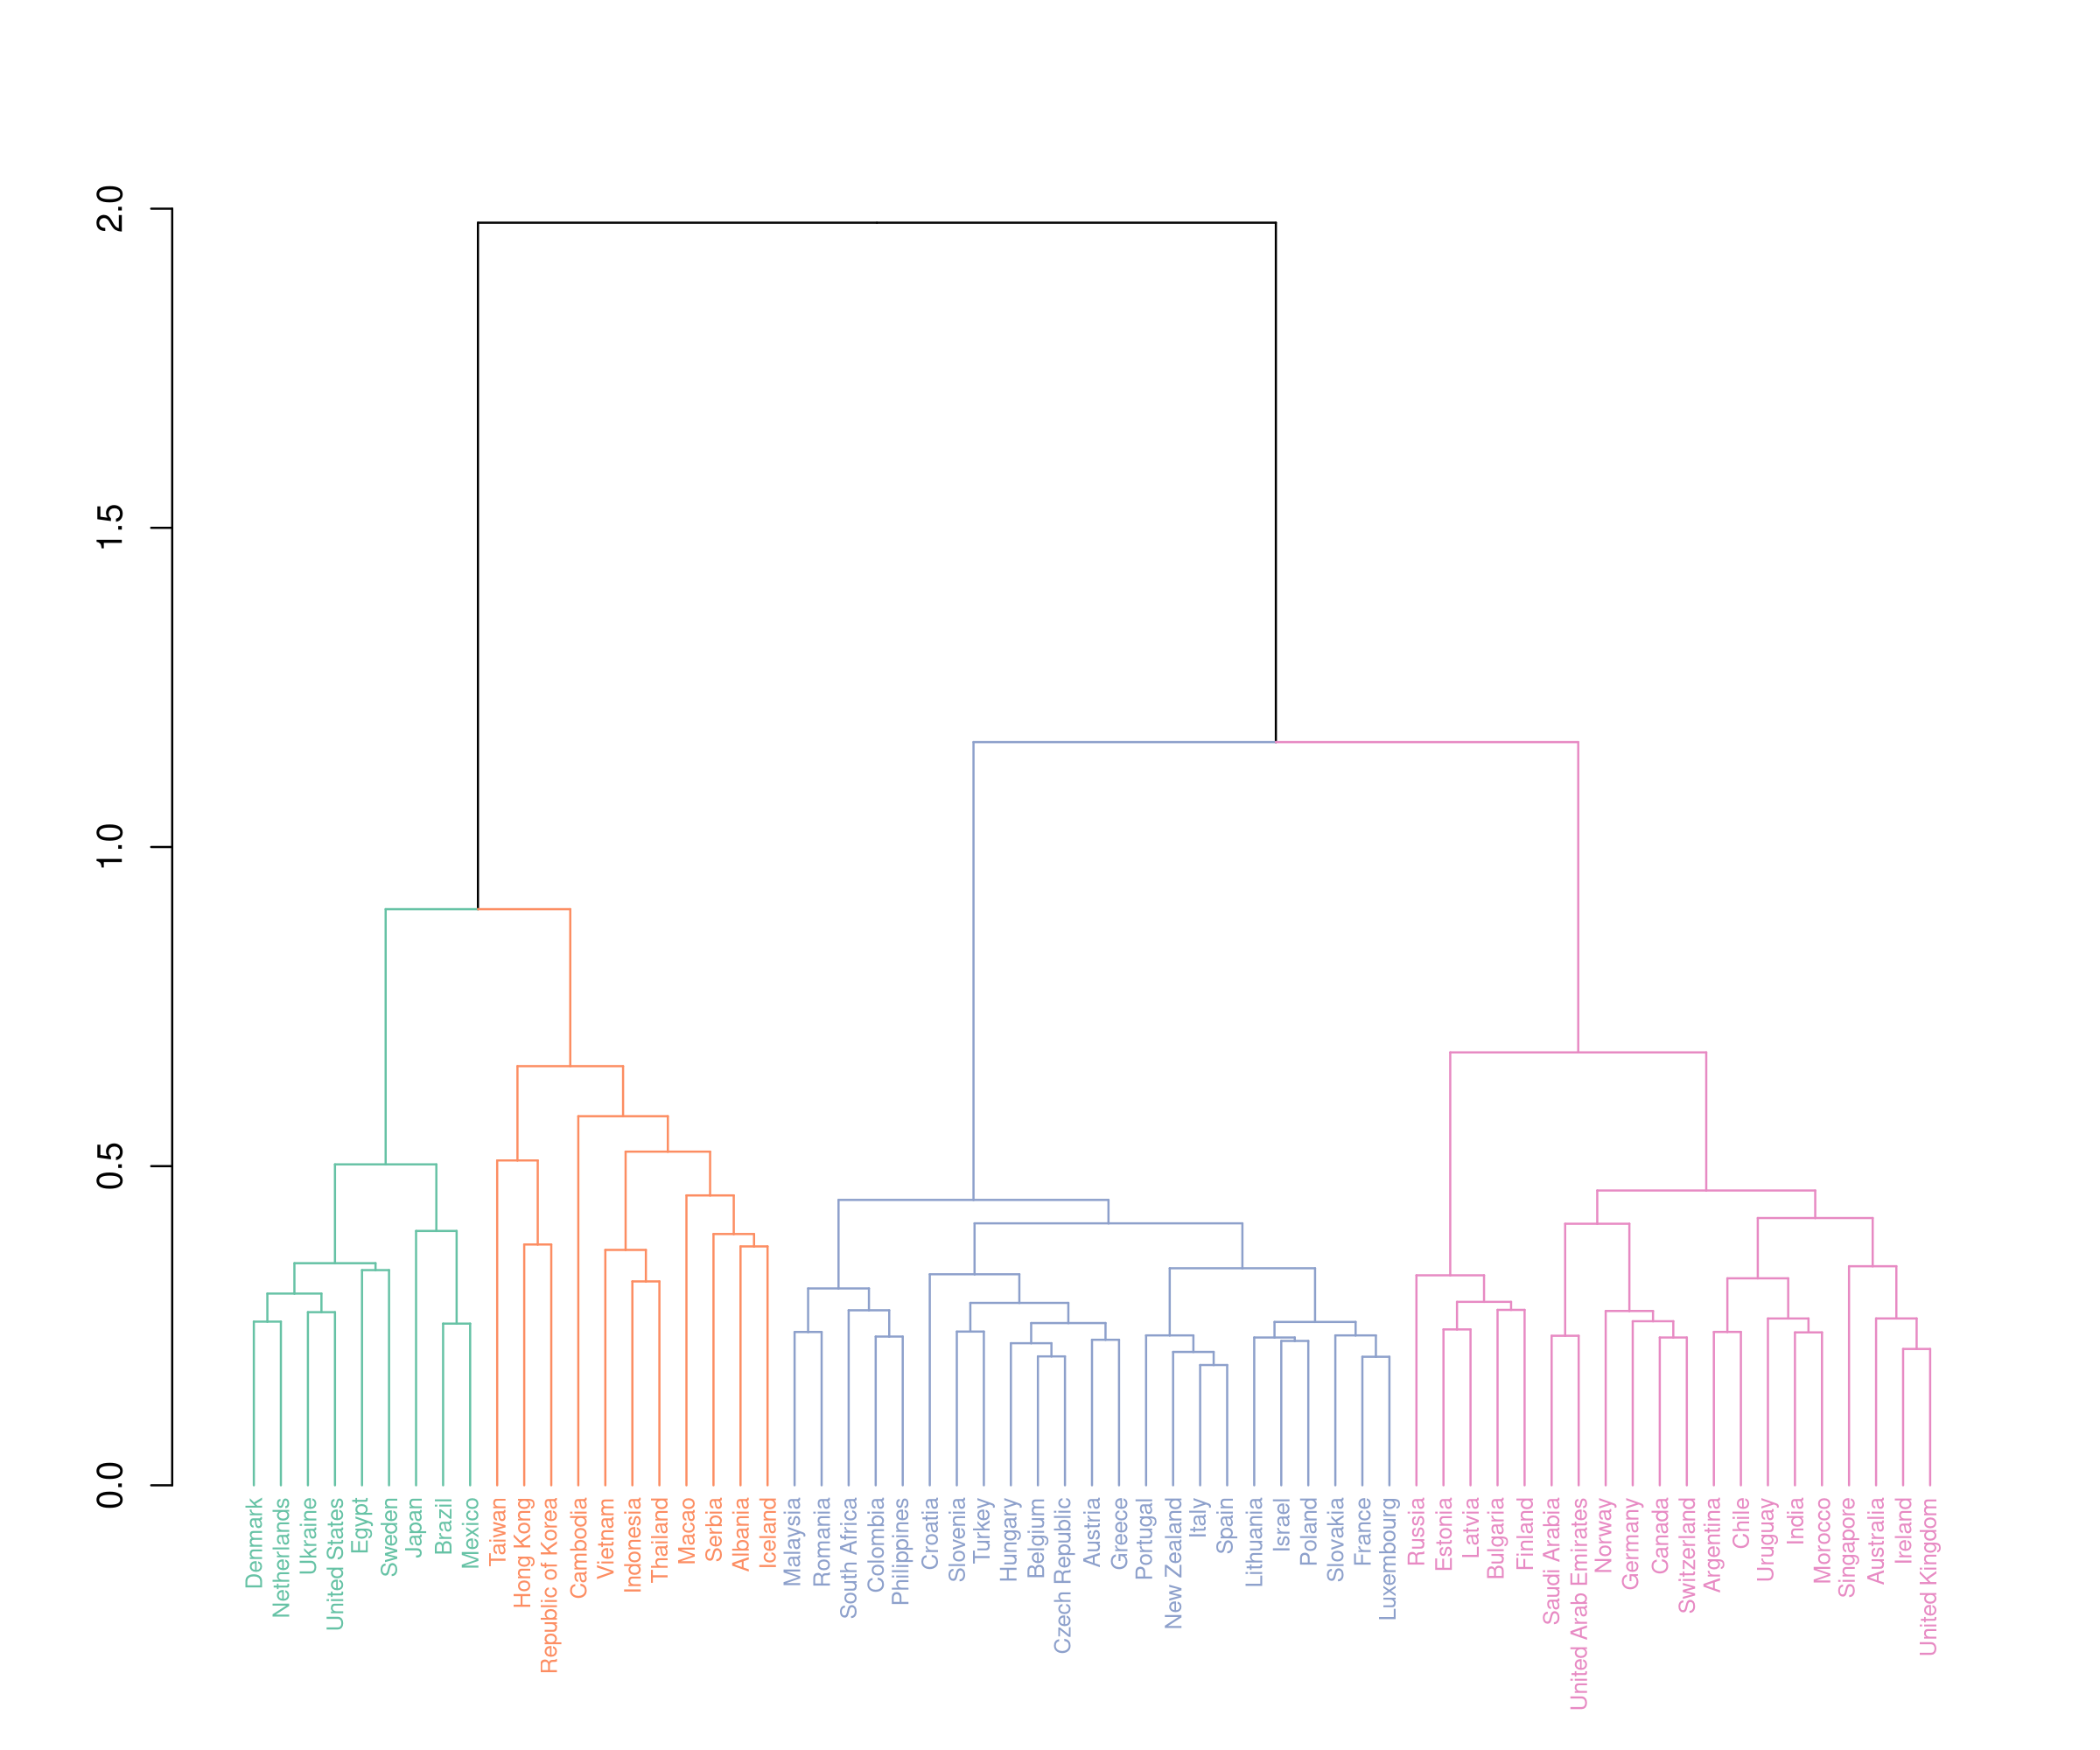
\includegraphics[width=\textwidth,trim={0cm 0 1.9cm 7cm},clip]{dendrogram}
  \caption{Dendrogram indicating four clusters of countries based on nine mobility and activity indicators}
  \label{fig:dend}
\end{figure}

We then plot the trends of activity changes as observed from Google location data, grouping these by cluster (\autoref{fig:act}).
Trends are shown by means of a generalized linear model estimated for each country.
Except in Cluster 1, which consists notably of South Korea, Hong Kong, Taiwan and Vietnam (countries with some of the best COVID-19 outcomes),
there was a significant downturn in work activities from mid-February to early April.
This decrease is as great as 75 percentage points in Clusters 2 and 3.
However, in Cluster 4 (e.g.\ United States, Brazil, Japan), it only reaches 50 percentage points.
The change in work activities can be seen as a partial indicator of lockdown policies or behavioral responses to the pandemic in each of the countries.
Transit activities similarly reduced in Clusters 2 and 3, but not as severely in Cluster 4.
Notably, in Cluster 1, transit stop activities dipped the lowest in South Korea compared to the other countries.
This outcome can be readily understood given that South Korea focused heavily on contact tracing to mitigate the spread of COVID-19 \cite{aum2020covid19,parkearly}.

Grocery shopping experienced a downturn in most countries. However, Clusters 1 and 4 show the smallest disruptions (a decline of about 20 percentage points).
The same trend is observed for retail activities.
However, in Cluster 4, this category had a more severe downturn (as many as 60 percentage points from the baseline), compared to grocery shopping.
This could be explained by policies keeping grocery stores open as essential services, while other retail outlets were shut.
Also, home activities (people staying in their places of residence) increased across all countries, peaking in April and then declining thereafter.
The change from baseline was greatest in Cluster 3 (generally over 50 percentage points), indicating that countries in this cluster stayed at home the most.
Furthermore, the peak for home activities occurs the latest in Cluster 3.

There are no discernible cluster-specific patterns for park activities for Clusters 1, 2 and 4 (as trends vary by country).
However, in Cluster 3, many countries observed a decline of up to 75 percentage points through April, followed by a large uptick.

% \begin{figure}[h!]
%   \centering
%   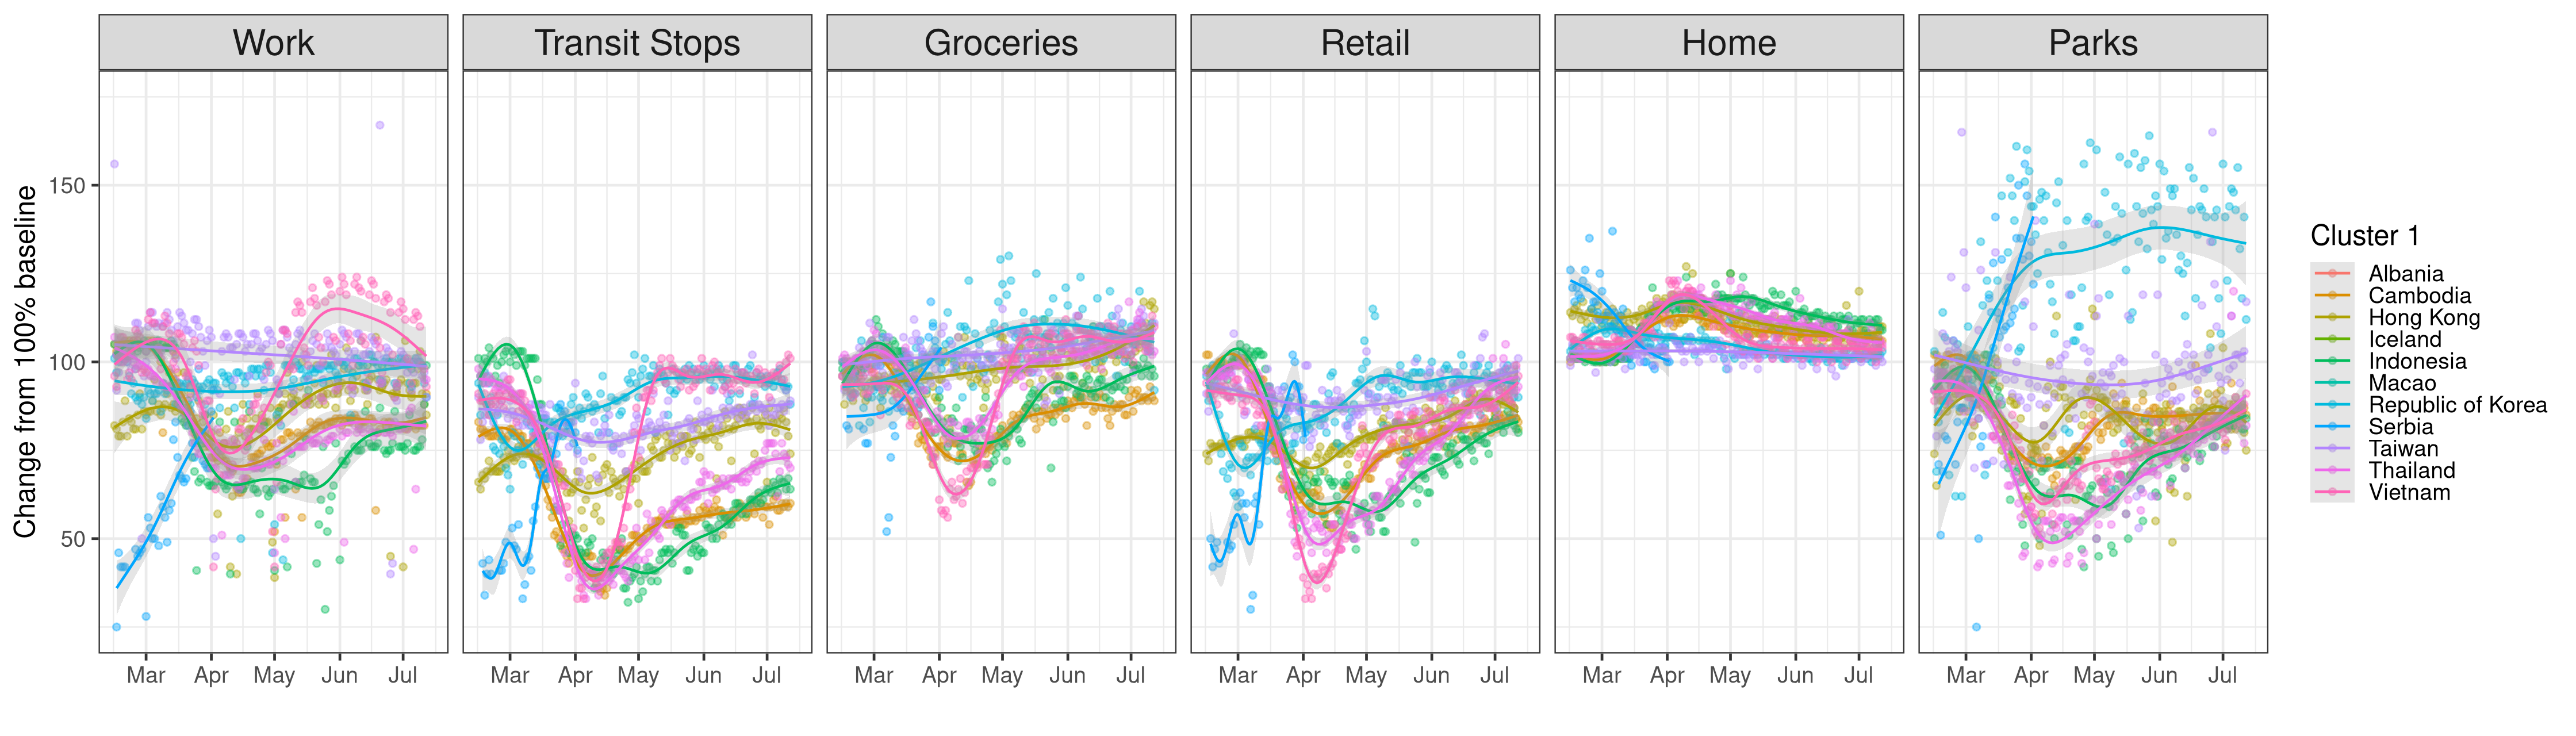
\includegraphics[width=\textwidth]{c1-activity}
%   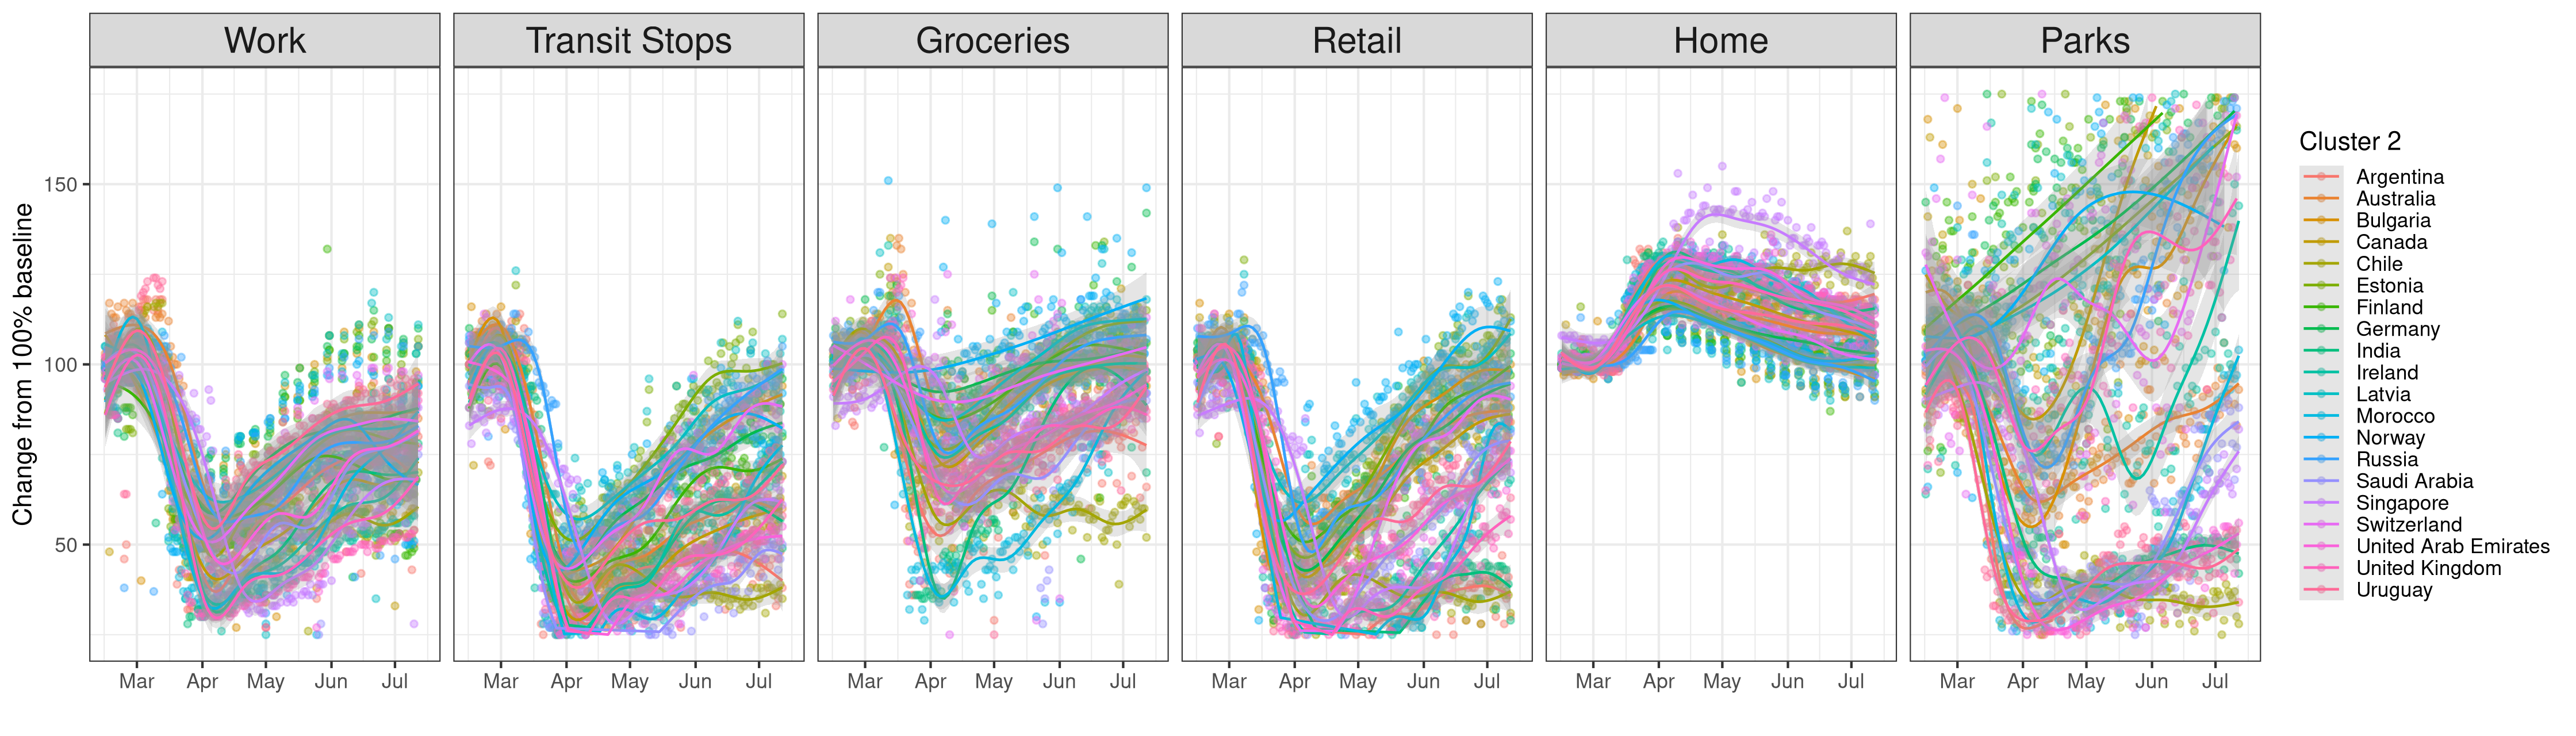
\includegraphics[width=\textwidth]{c2-activity}
%   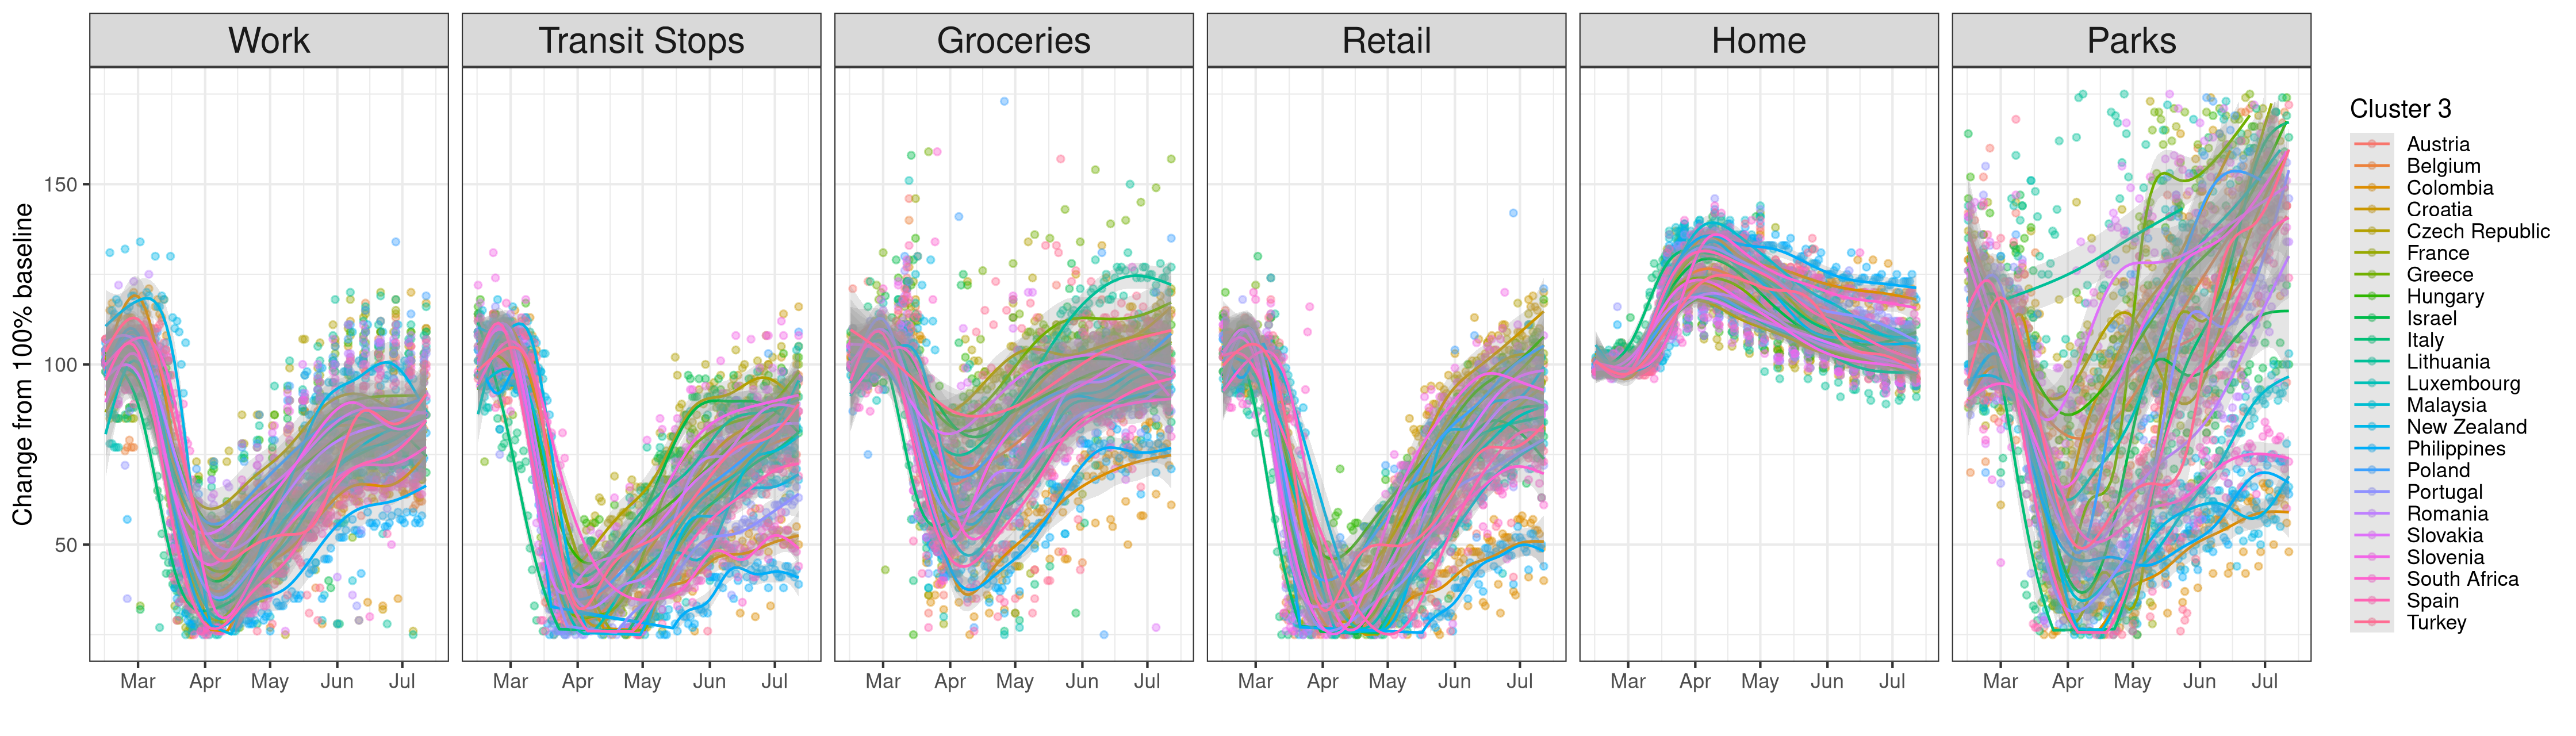
\includegraphics[width=\textwidth]{c3-activity}
%   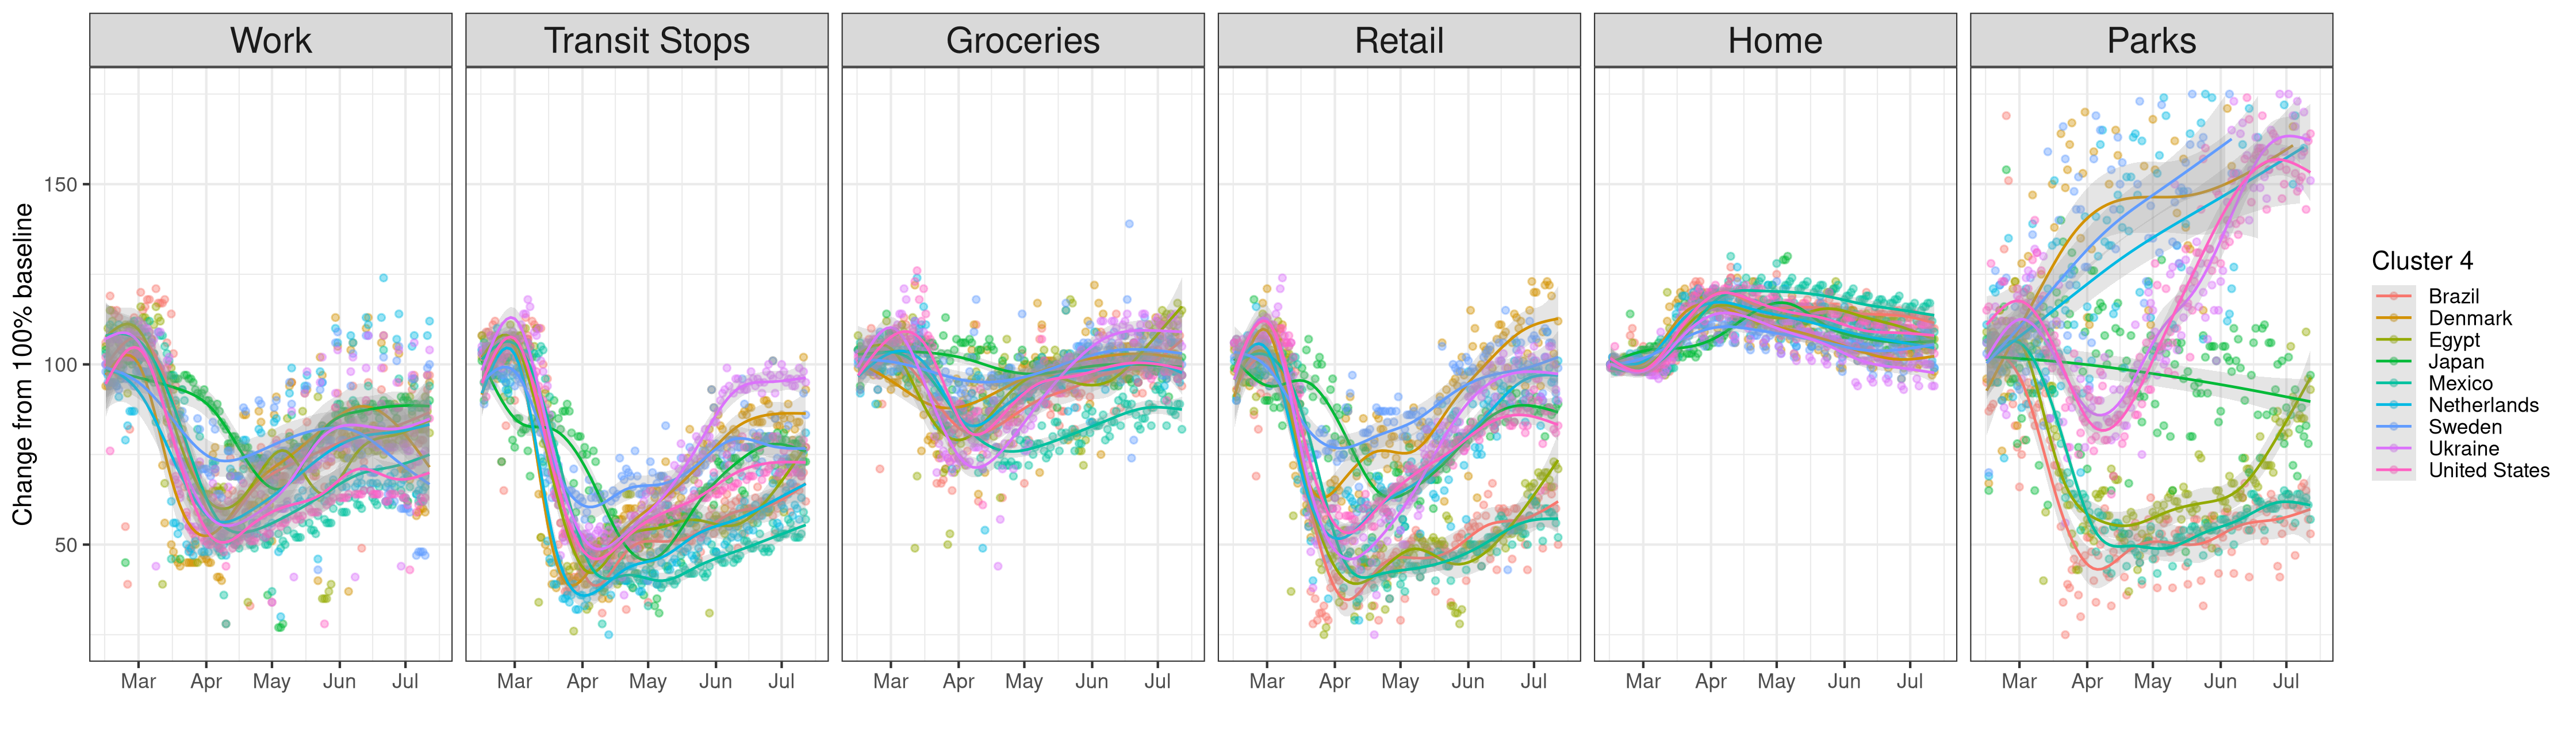
\includegraphics[width=\textwidth]{c4-activity}
%   \caption{Activity changes from baseline (100\%) by cluster (Google dataset).  Trends are indicated using a generalized linear (GLM) fit for each country.}
%   \label{fig:act}
% \end{figure}


% The driving, transit and walking activities observed from navigation via Apple devices do not distinctly vary among the clusters (\autoref{fig:mob}).
% This could be explained by the fact that usual activities perhaps do not require navigation.
% And also since Apple Maps users are not always representative of the population, it is less likely that changes in regular activities would be discernible from these data.

% \begin{figure}[h!]
%   \centering
%   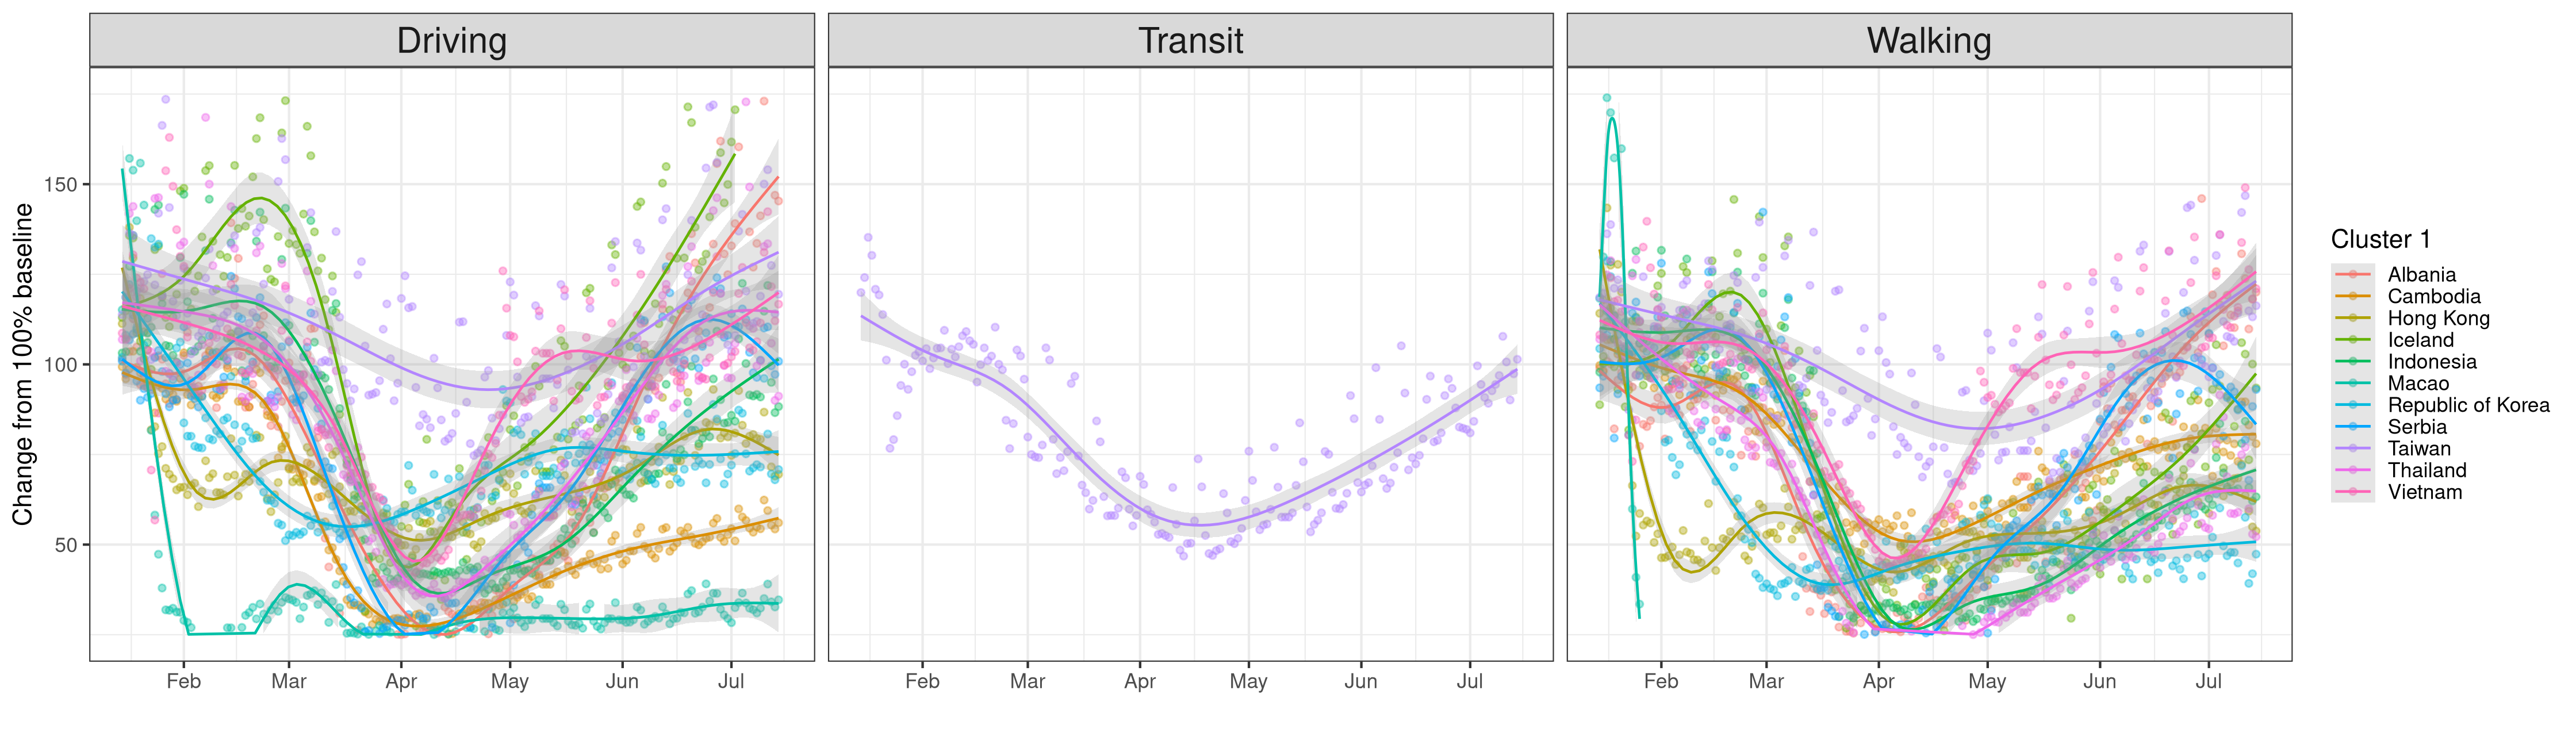
\includegraphics[width=.9\textwidth]{c1-mobility}
%   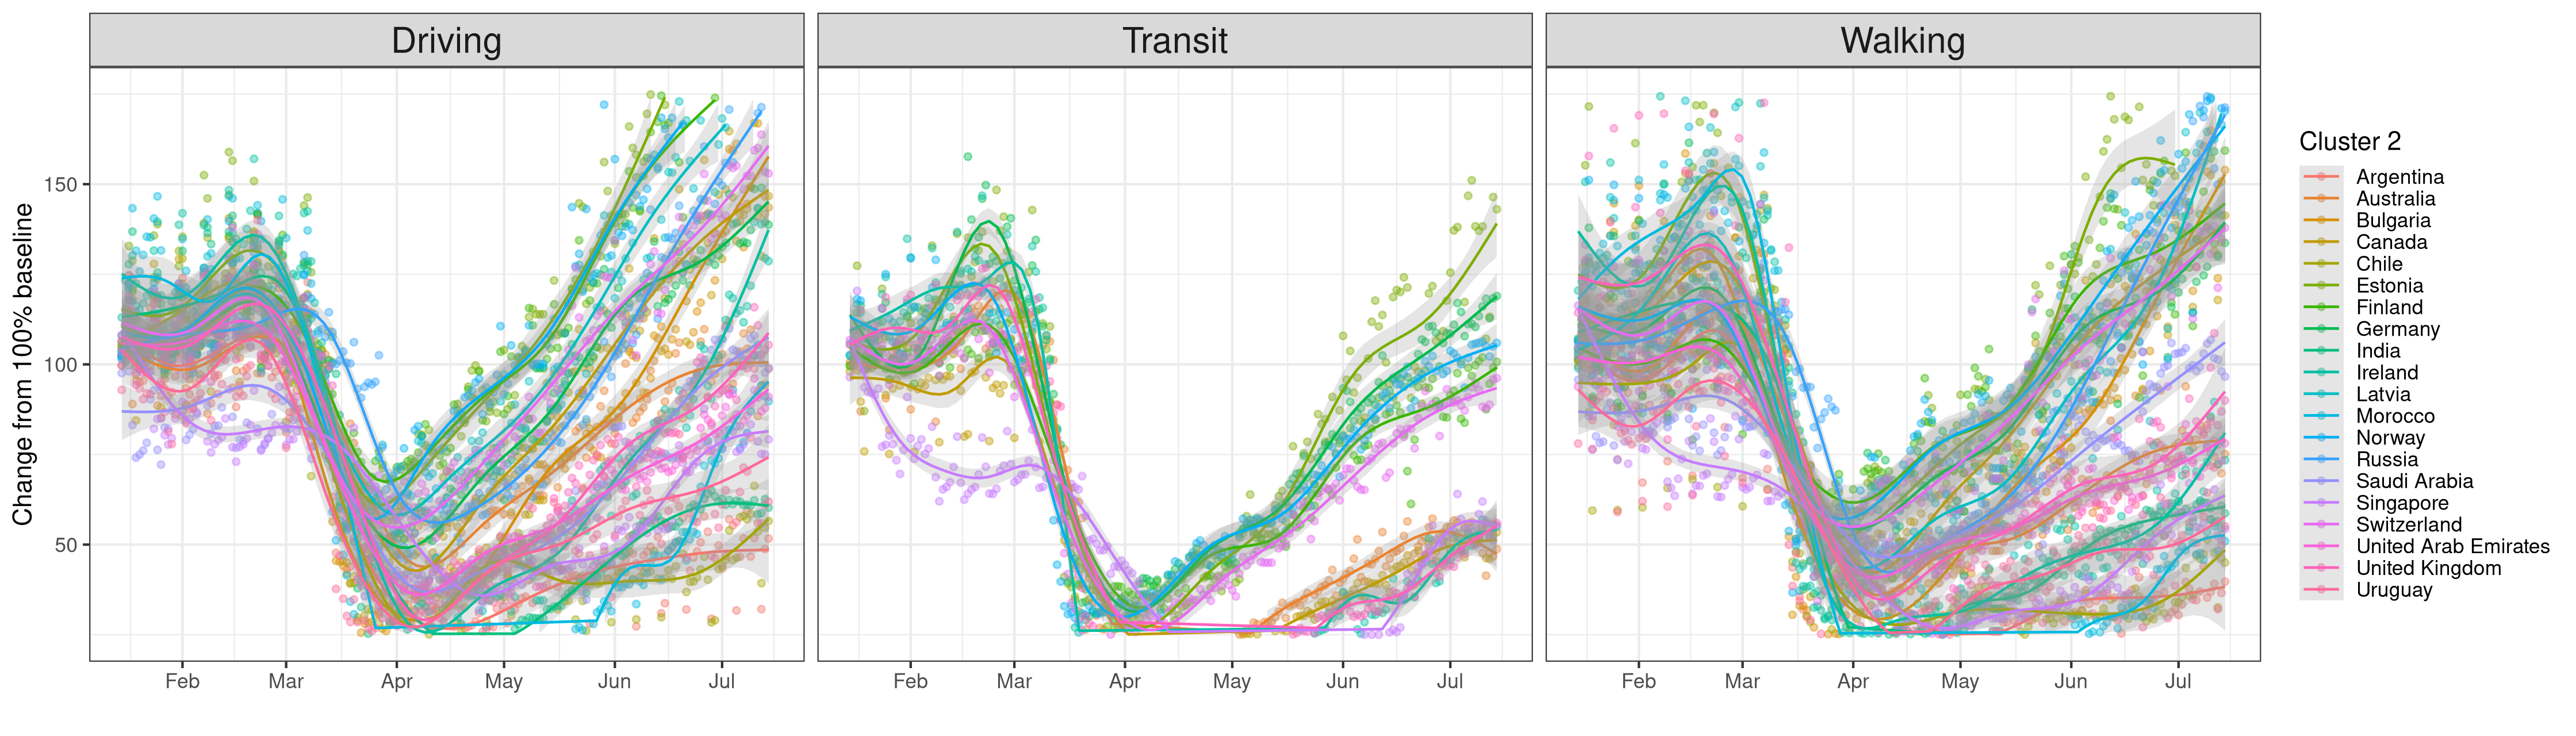
\includegraphics[width=.9\textwidth]{c2-mobility}
%   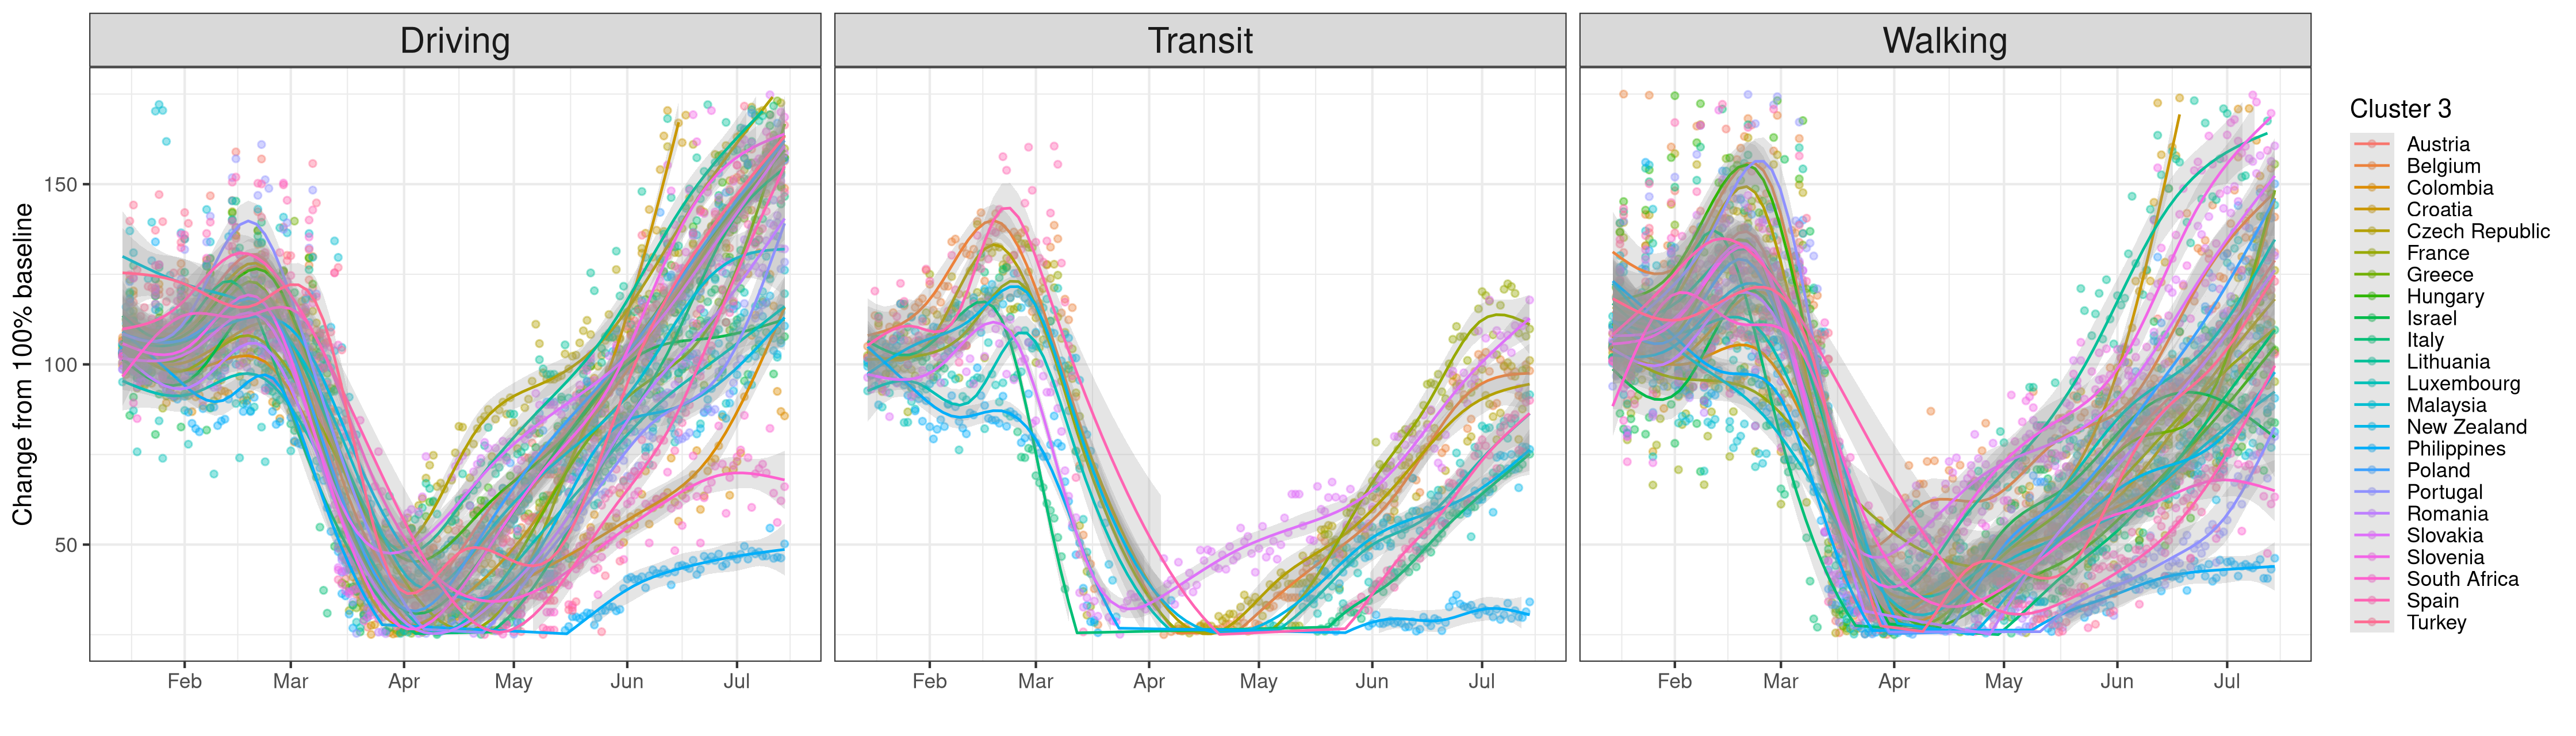
\includegraphics[width=.9\textwidth]{c3-mobility}
%   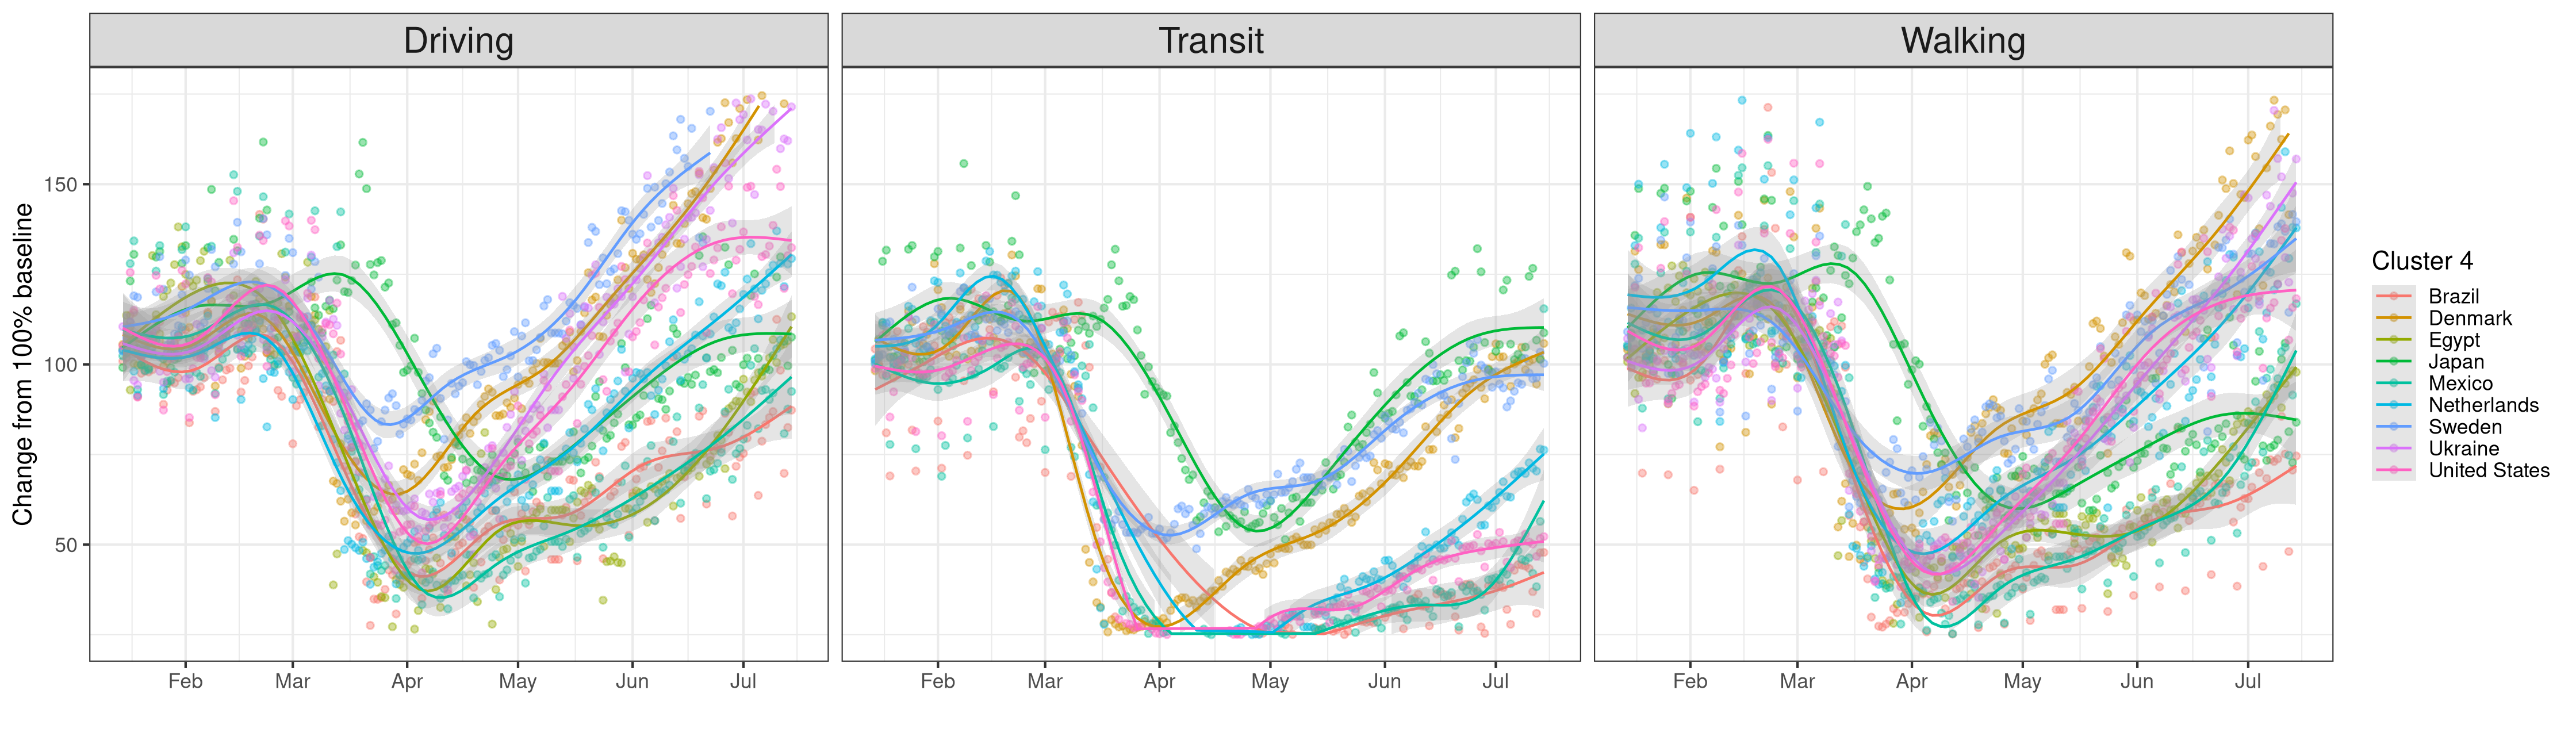
\includegraphics[width=.9\textwidth]{c4-mobility}
%   \caption{Mobility changes from baseline (100\%) by cluster (Apple dataset). Trends are indicated using a generalized linear (GLM) fit for each country.}
%   \label{fig:mob}
% \end{figure}


We show the daily confirmed COVID-19 cases at the country level by cluster in \autoref{fig:cov} on a log-y scale.
Most of the countries in Cluster 1 have experienced a decrease in COVID-19 cases.
However, Serbia and Indonesia are outliers.
Given that the countries in this cluster had the least disruption in activities compared to other clusters, other exogenous factors are probably responsible for the favorable COVID-19 outcomes.
Clusters 2 and 3 were harder hit in the early weeks of the year, but indicate a downturn in COVID-19 infections from late March and early April.
These clusters had the most severe decreases in work and transit activities (and highest increases in home activities) from the baseline.
Clearly, there are few exceptions in each of these clusters, such as India in Cluster 2 and Colombia in Cluster 3.
Finally, in Cluster 4, most of the countries have been on an upward trajectory in recent weeks (except for Denmark).
In these countries, there is evidence of lockdowns being lifted too soon and perhaps less strict public health policies than elsewhere.
In terms of activities, this is one cluster where home activities showed the least disruption, which is an indicator of the aforementioned trend.

\begin{figure}[h!]
  \centering
  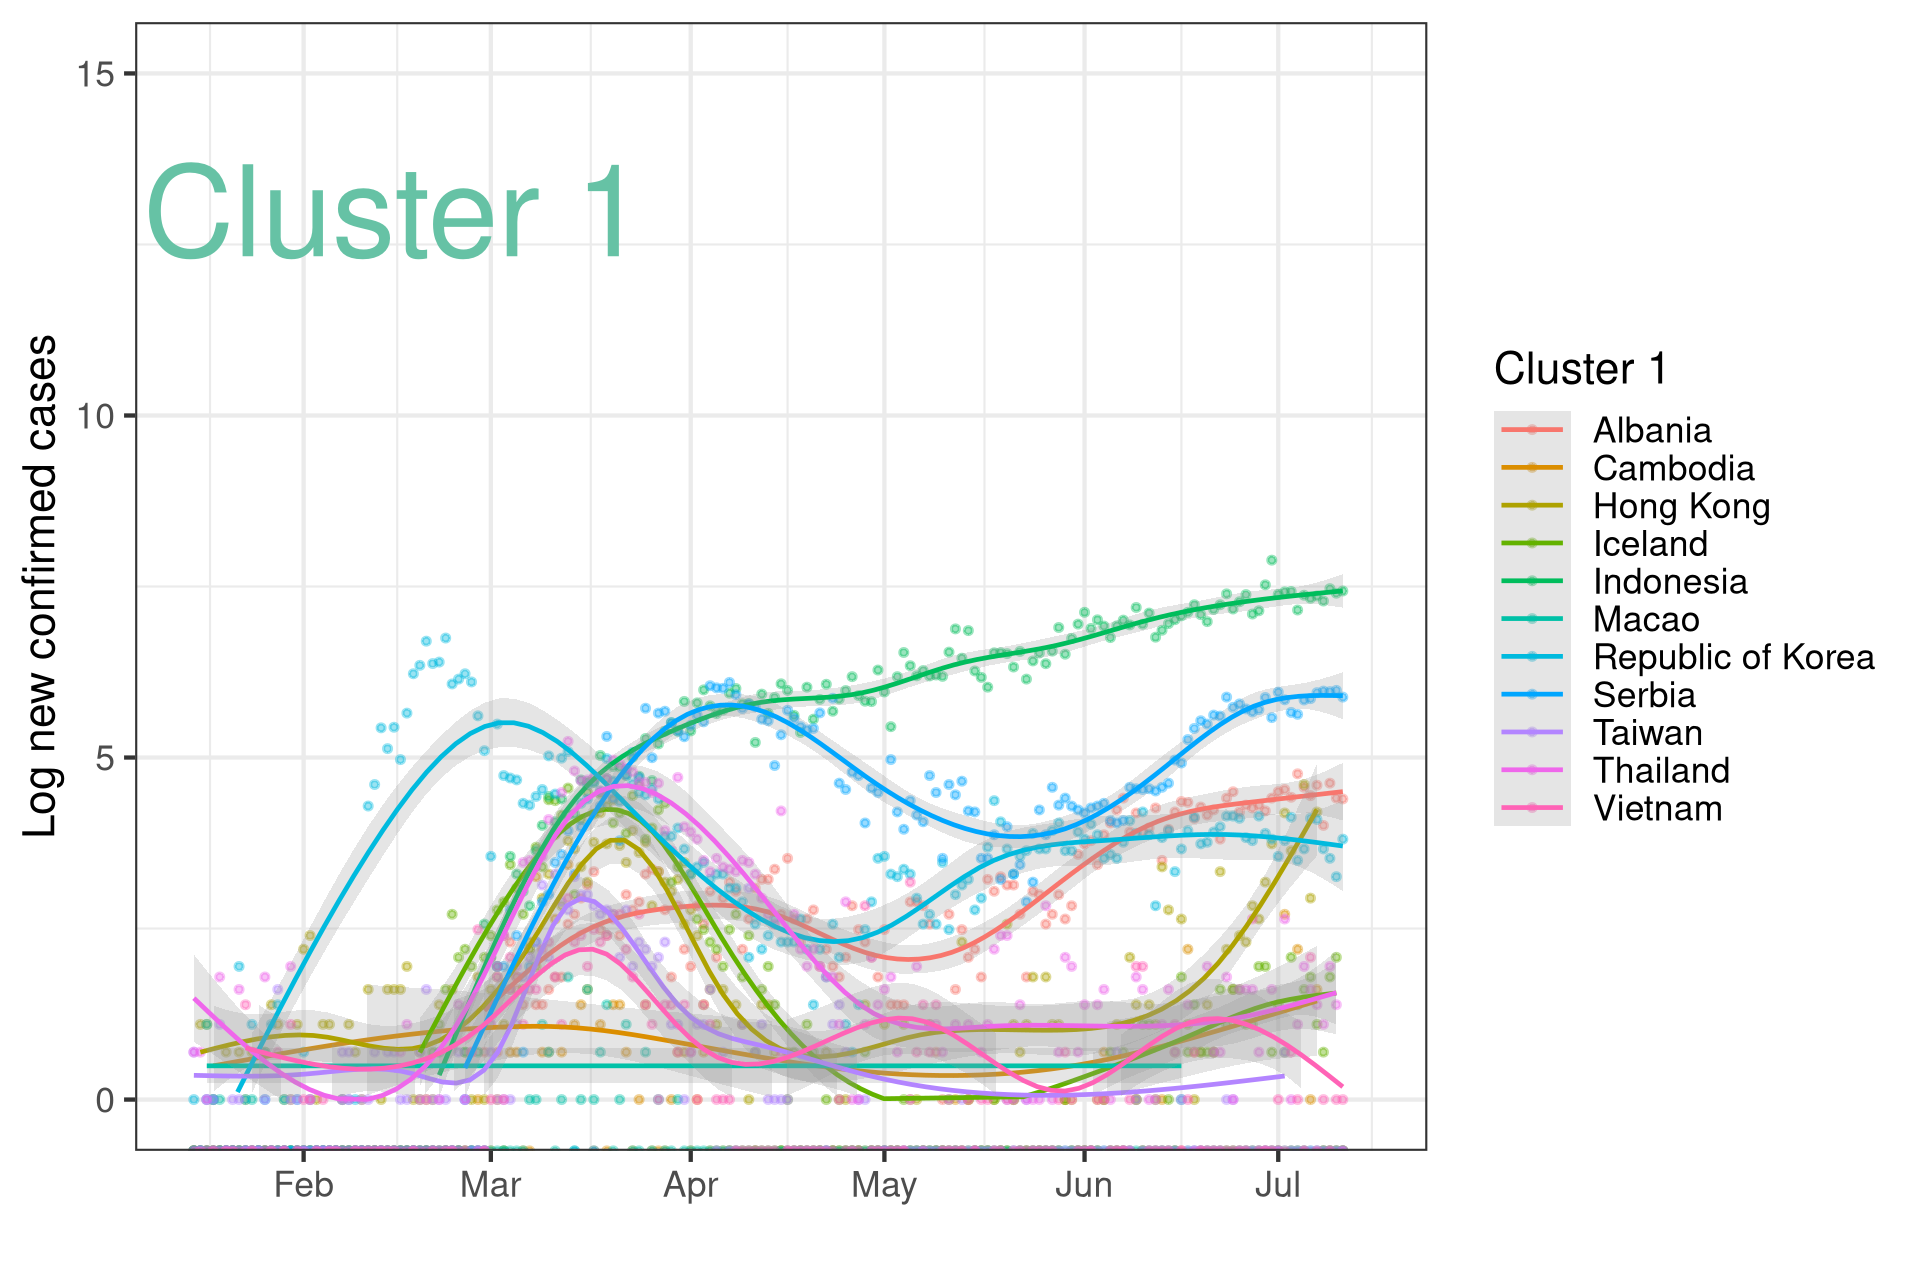
\includegraphics[width=.45\textwidth]{c1-cov}
  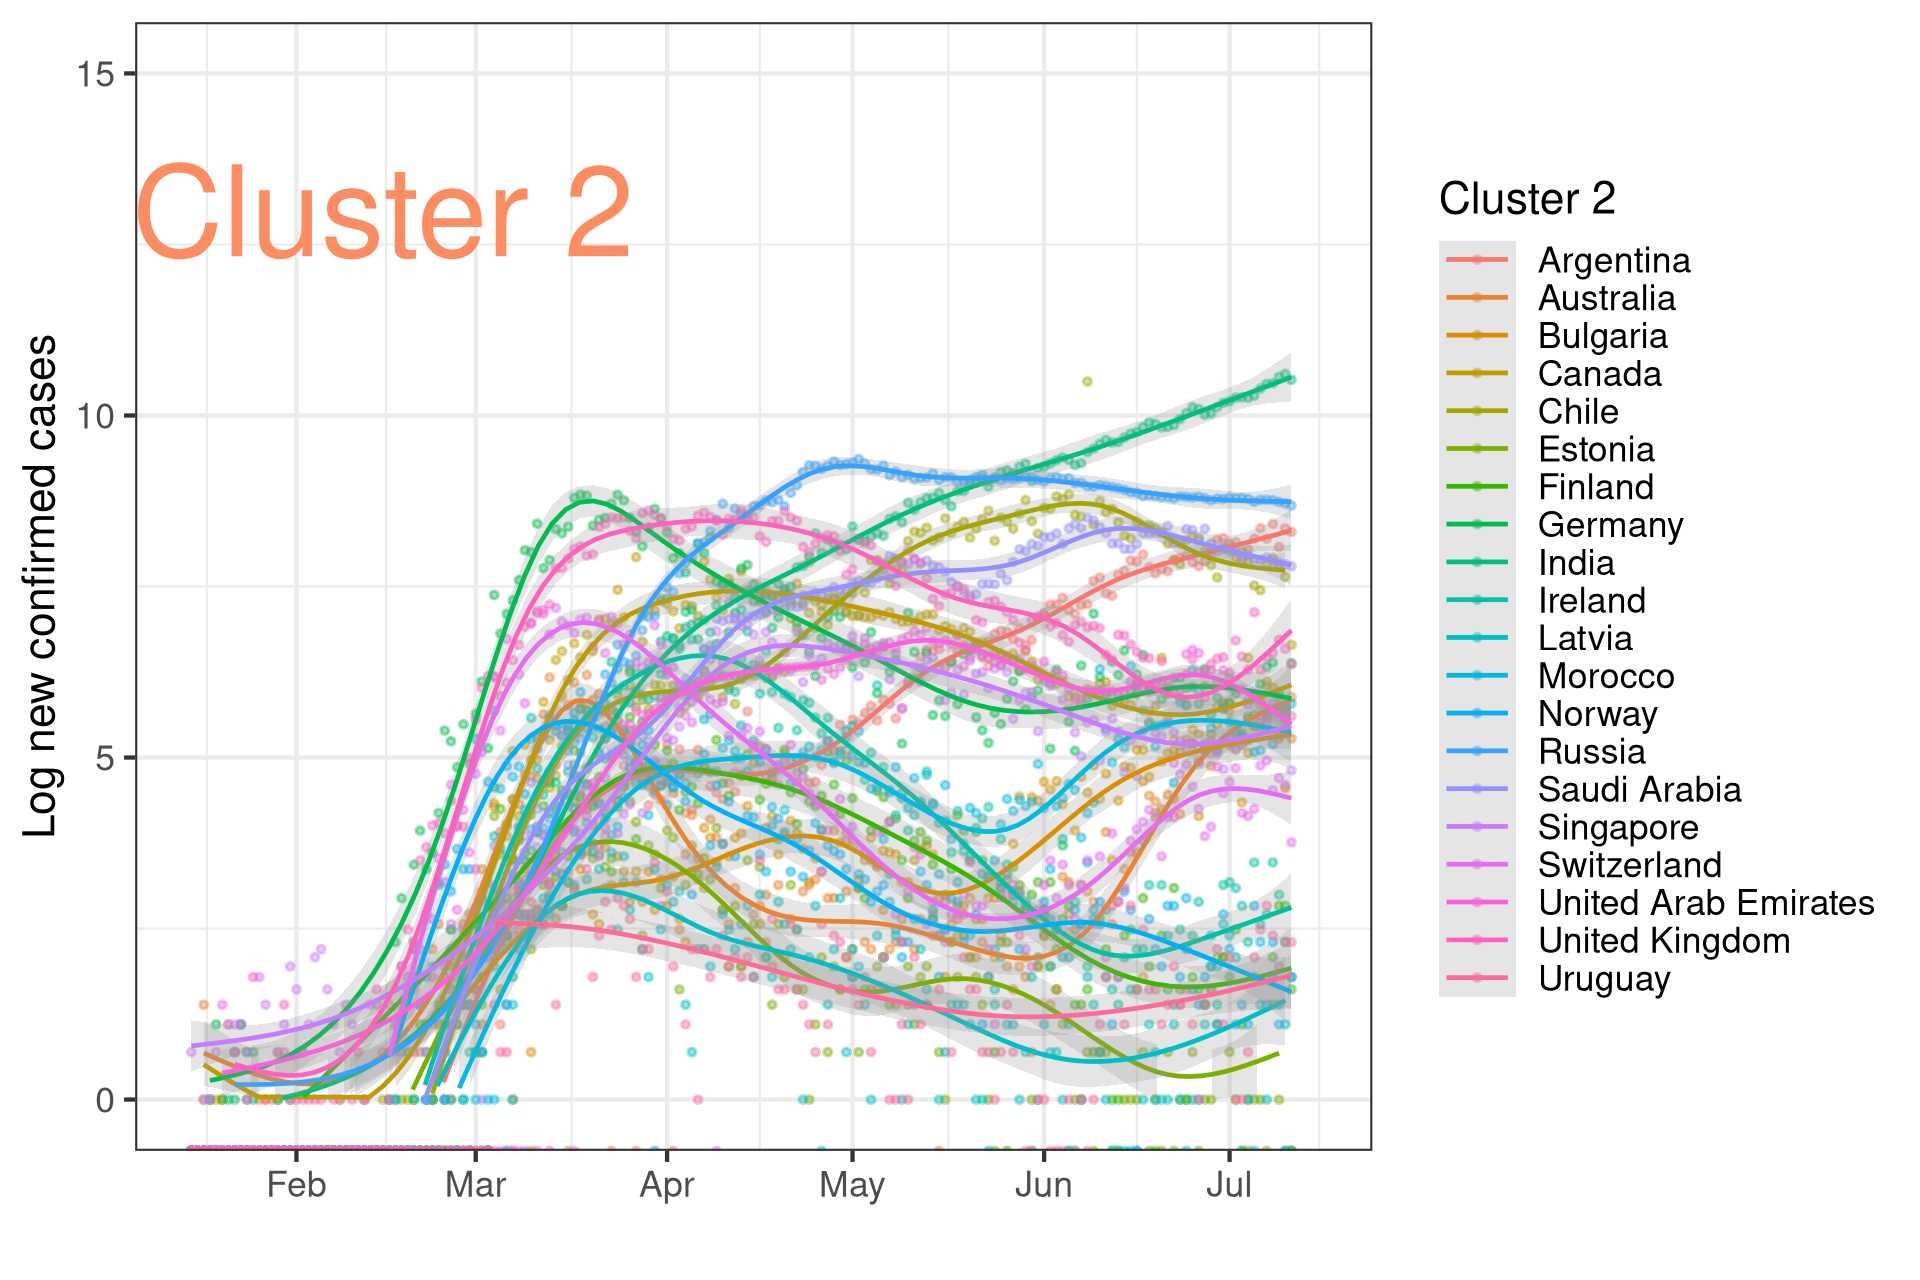
\includegraphics[width=.45\textwidth]{c2-cov}
  
  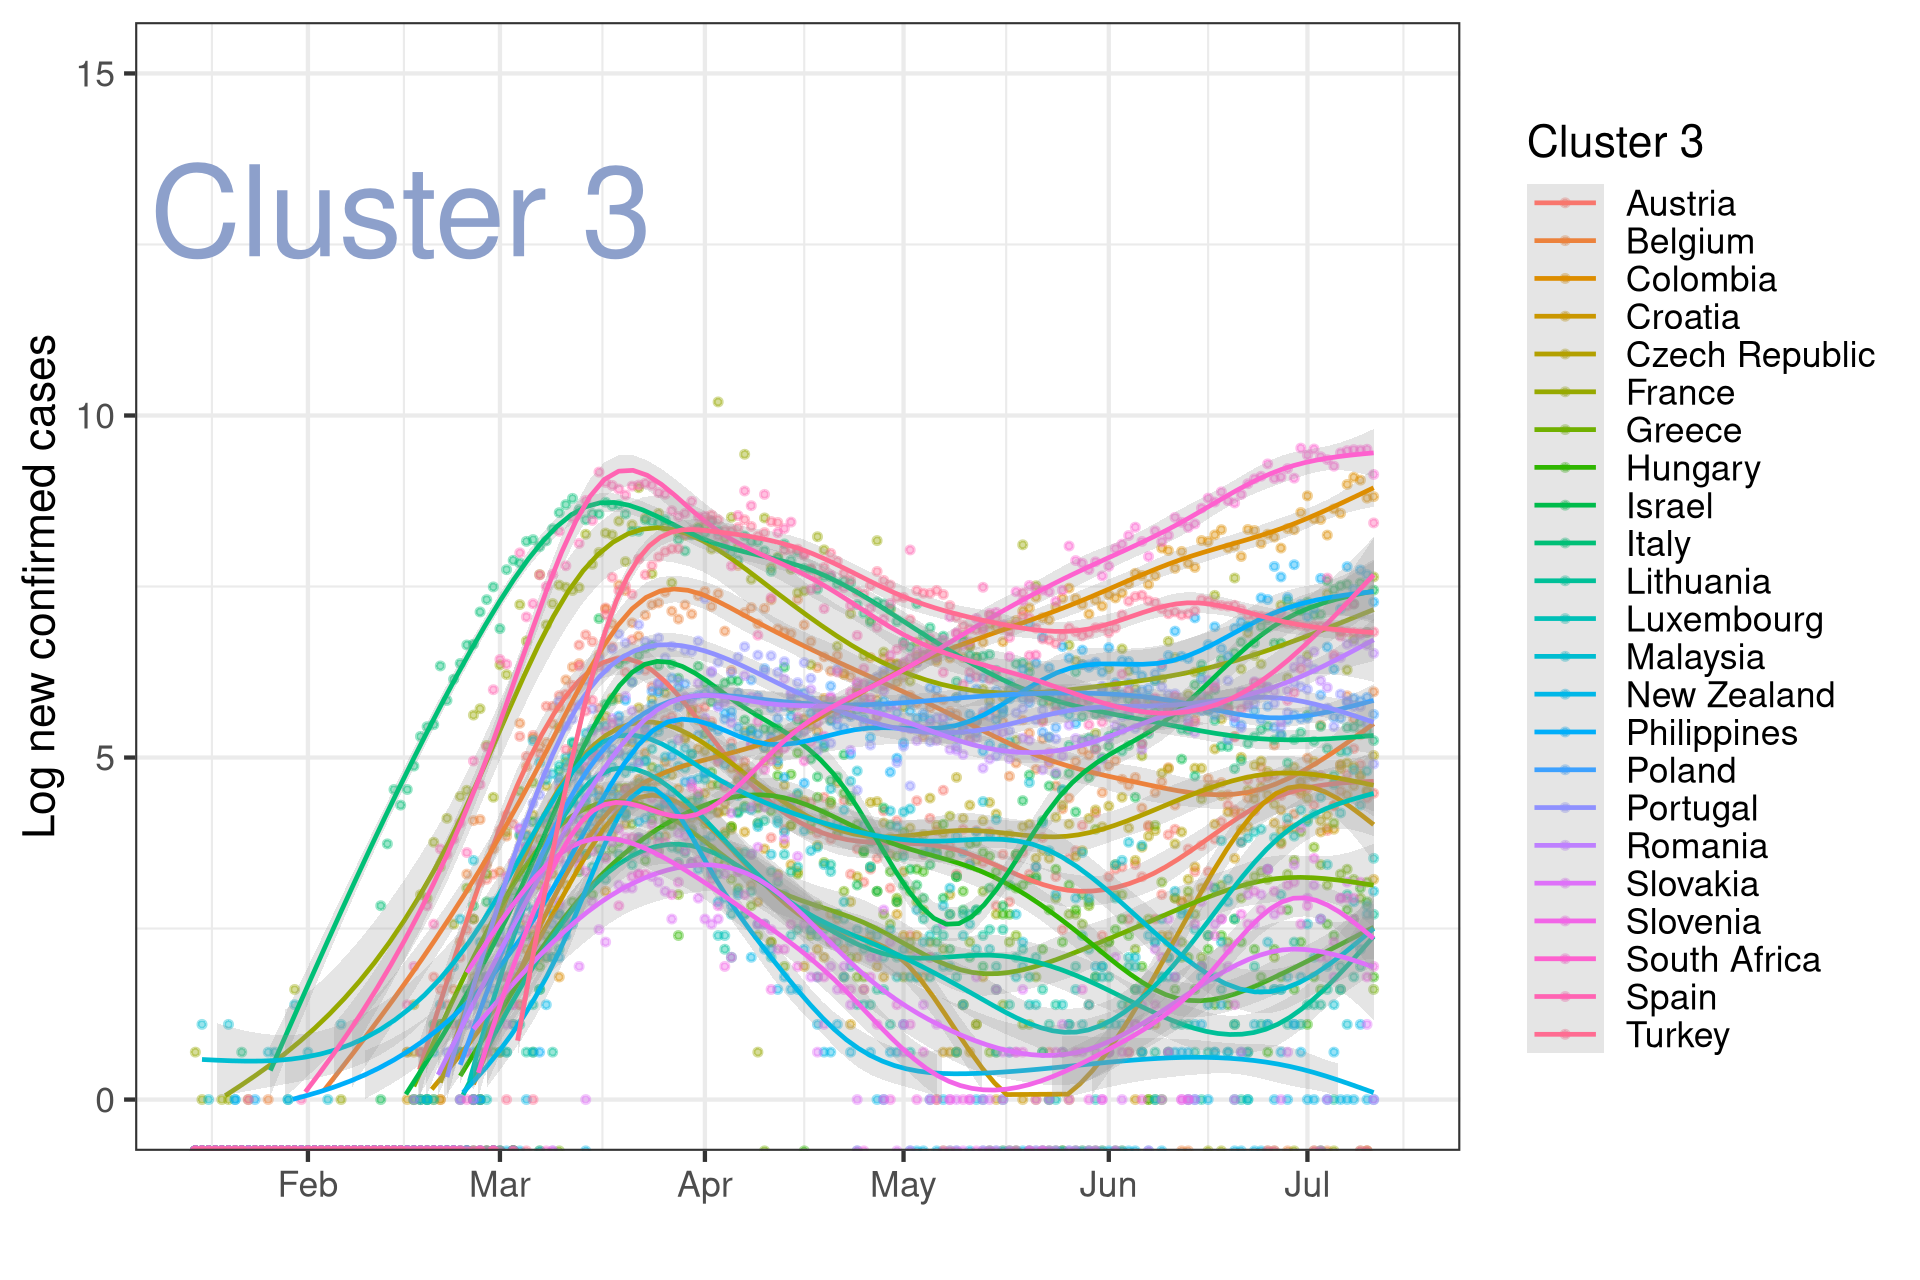
\includegraphics[width=.45\textwidth]{c3-cov}
  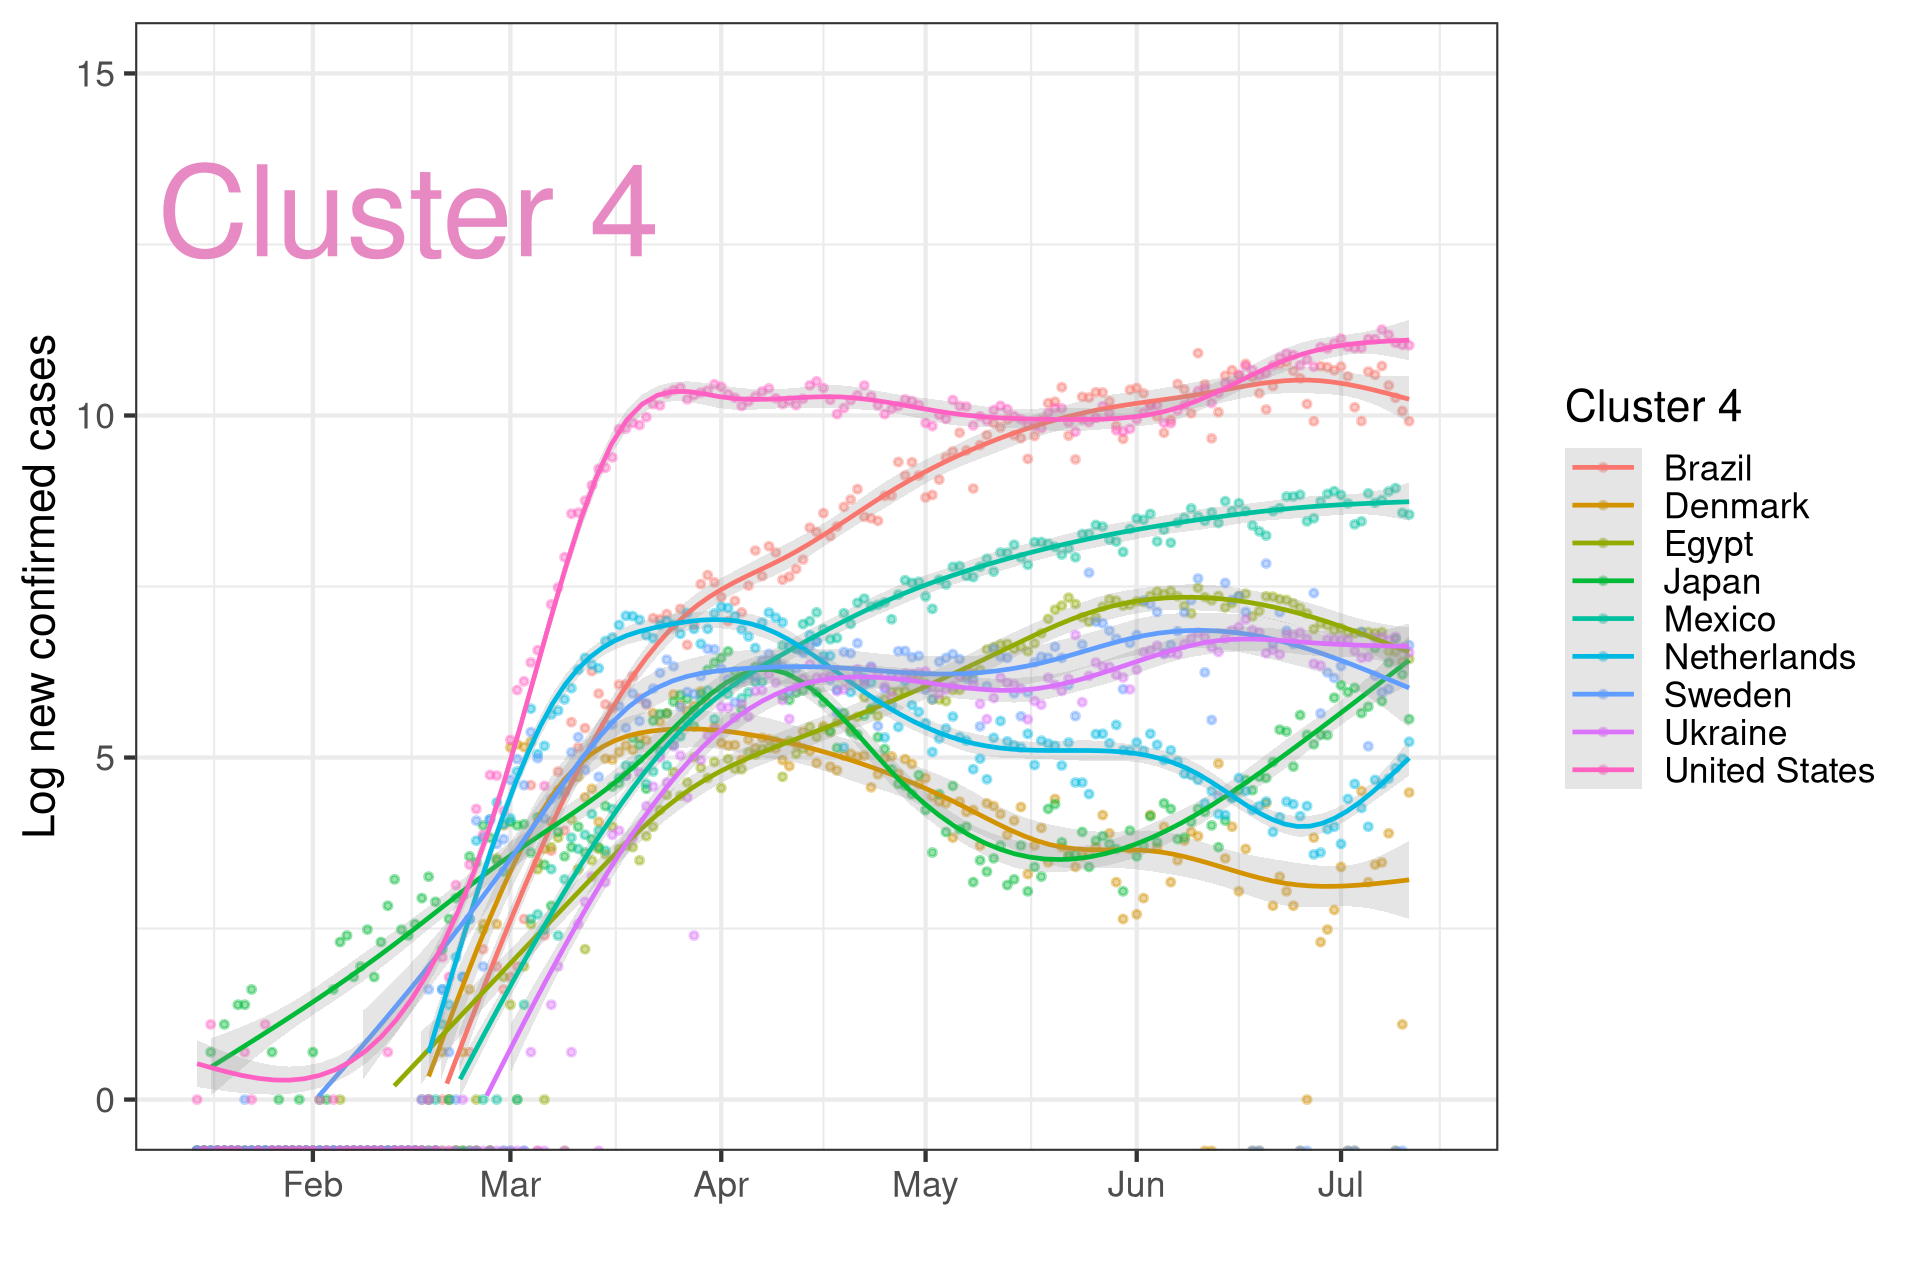
\includegraphics[width=.45\textwidth]{c4-cov}
  \caption{Daily confirmed COVID-19 cases for each of the clusters (log y-axis); Johns Hopkins dataset.}
  \label{fig:cov}
\end{figure}


\subsection{Expected results}
We plan to estimate country-level vector autoregression models (VARs), cluster-level panel VARs and a global VAR.
These models will enable us to explain how COVID-19 outcomes were impacted by changes across these activities.
They would also allow us to analyze how changes in one dimension would affect the other (using impulse response functions).
Other variables that can explain COVID-19 impacts (particularly interventions) will be included in these models as strictly exogenous variables.
Air passenger travel flows will also be incorporated as weights on weakly exogenous (foreign) variables in the global VAR model.
These would allow the inclusion of the effects of observations in other countries across these dimensions.


\section{Discussion}

\section{Conclusion }
We cluster the countries in our sample into four categories based on similar activity and mobility trends.
% By running the model with a different lag parameter for each country we attempted to estimate the optimal lag for each country.
% However, our VAR implementation fell short of producing statistically significant results.
Future work will focus on estimating VAR models for each of the countries, adding exogenous and weakly exogenous variables such as interventions and restrictions (social distancing orders, travel bans, etc.), as well as deterministic ones (country characteristics).
Subsequently, cluster-level VARs and a global VAR will be estimated.
These models will provide insights into the processes governing the changes in the endogenous variables (COVID-19 outcomes, activity and mobility trends), as well as potential forecasting capabilities.
The insights gained from these models would enable policy and decision makers plan efficiently for recovery from the current pandemic, as well as better prepare for future ones, by tailoring interventions relevant to the behavioral profiles of their respective countries.
%We also plan to substitute the number of new cases with a moving average for new COVID-19 cases which would produce more robust results.
 
% \section{Author Contribution Statement}
% The authors confirm contribution to the paper as follows: \\
% Study conception and design: \\
% Analysis and interpretation of results: \\
% Manuscript preparation:

%\section{Acknowledgment}

\bibliographystyle{elsarticle-num}
\bibliography{references.bib}


\end{document}

%%% Local Variables:
%%% mode: latex
%%% TeX-master: t
%%% End:

